\chapter{Transistor Biasing}\label{chap4}

\medskip

Biasing\index{Transistor!biasing} of transistor means to establish the required dc currents and voltages in the transistor circuit so that the transistor operates in the appropriate region of its characteristics for an intended application. Biasing\index{Biasing} circuits use dc sources and resistors for the purpose of biasing. A variety of biasing circuits exist. Among them, base bias is the simplest and voltage divider bias is the best. This chapter starts with the concept of dc load line, $Q$ point and fixing of $Q$ point on dc load line. The analysis and design of base bias and voltage divider bias have also been studied.

\section{Need for biasing}\label{sec4.1}

The transistor needs to be operated in an appropriate region of characteristics depending upon the application of the circuit in which it is used.

\vskip .1cm

When the transistor is to be used as an amplifier, it must be operated in the active region of its characteristics i.e., its base-emitter junction should be forward biased and collector base junction should be reverse biased. On the other hand, the transistor is operated between cut-off and saturation, when it is used as a switch.

\vskip .1cm

Biasing circuits employ a resistive network and a dc power supply to establish the required dc currents and voltages in the transistor circuit.

\subsection{DC load line}\label{sec4.1.1}

The DC load line\index{DC load line}\index{Transistor!dc load line} for a transistor circuit is a straight line drawn on the transistor output characteristics. For a common emitter (CE) circuit, the load line is a graph of collector current $(I_{C})$ versus collector-emitter voltage $(V_{CE})$, for a given value of collector resistance $(R_{C})$ and a given supply voltage $(V_{CC})$. The load line shows all corresponding levels of $I_{C}$ and $V_{CE}$ that can exist in a particular circuit.

\subsection{Procedure for drawing the DC load line on the transistor CE output characteristics}\label{sec4.1.2}
\index{DC load line!procedure for drawing}

Consider an $npn$ transistor in CE configuration biased in the active region as shown in Fig.~\ref{fig4.1}.
\begin{figure}[H]
\centering
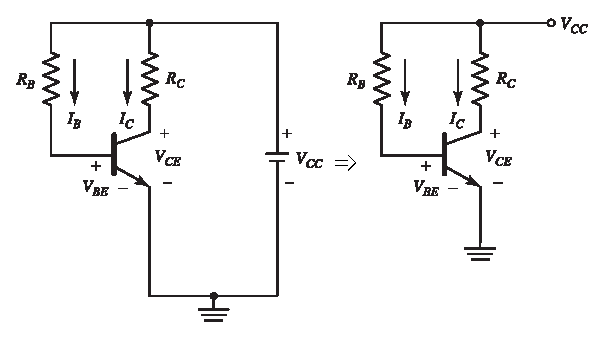
\includegraphics{chap3/S3-EE-03-035.eps}
\caption{Transistor in CE configuration biased in the active region}\label{fig4.1}
\end{figure}

The $dc$ supply voltage $V_{CC}$ forward biases the emitter-base junction and reverse biases the collector-base junction. Applying Kirchhoff's Voltage Law to the base-emitter circuit we have,
\begin{align}
\text{supply voltage} &= \text{voltage across $R_{B}\,+\,$ Base-emitter voltage $V_{BE}$}\notag\\[3pt]
\text{i.e.,}\qquad V_{CC} &= I_{B}R_{B}+V_{BE}\notag\\[3pt]
\Rightarrow I_{B} &= \frac{V_{CC}-V_{BE}}{R_{B}}\label{eq4.1}
\end{align}

The collector current is given by,
\begin{equation}
I_{C}=h_{FE}I_{B}\label{eq4.2}
\end{equation}

Applying Kirchhoff's Voltage Law to collector-emitter circuit we have,
\begin{align}
\text{Supply voltage} &= \text{voltage across $R_{C}\,+\,$ Collector-emitter voltage $V_{CE}$}\notag\\[3pt]
\text{i.e.,}\qquad V_{CC} &= I_{C}R_{C}+V_{CE}\label{eq4.3}
\end{align}

When $I_{B}$ is set to zero, $I_{C}$ becomes zero. From Eqn.~\eqref{eq4.3} we get $V_{CE}=V_{CC}$. The transistor is said to be at cut-off. The co-ordinates of the point say $A$ on the output characteristics corresponding to the cut-off of transistor, which is given by
\begin{equation}
A(V_{CE},I_{C})=A(V_{CC},0)\label{eq4.4}
\end{equation}

When the transistor is fully turned on by adjusting $I_{B}$ such that
\begin{align}
I_{C}R_{C} &= V_{CC}\notag\\[3pt]
\text{or}\qquad I_{C} &= \frac{V_{CC}}{R_{C}}\label{eq4.5}
\end{align}
the collector-emitter voltage from Eqn.~\eqref{eq4.3} is obtained as
\begin{equation}
V_{CE}=0\label{eq4.6}
\end{equation}

The transistor is said to be in saturation. The co-ordinates of the point say $B$ on the output characteristic, corresponding to the saturation of the transistor that is given by
\begin{equation}
B(V_{CE},I_{C})=B(0,V_{CC}/R_{C})\label{eq4.7}
\end{equation}

Let us mark these points on the CE output characteristics of the transistor. The straight line obtained by joining these points is called the DC load line and is shown in Fig.~\ref{fig4.2}.
\begin{figure}[H]
\centering
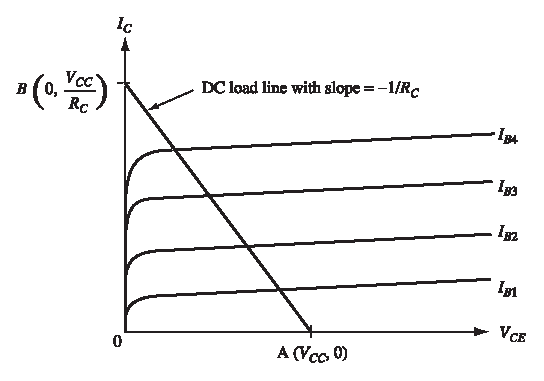
\includegraphics{chap3/S3-EE-03-036.eps}
\caption{DC load line drawn on transistor CE output characteristics}\label{fig4.2}
\end{figure}

The equation of DC load line can be obtained using Eqn.~\eqref{eq4.3}. That is,
\begin{align}
I_{C}R_{C} &= -V_{CE}+V_{CC}\notag\\[3pt]
I_{C} &= [-1/R_{C}]V_{CE}+\frac{V_{CC}}{R_{C}}\label{eq4.8}
\end{align}
Eqn.~\eqref{eq4.8} is of the form
\begin{equation}
y=mx+c\label{eq4.9}
\end{equation}

Comparing Eqns.~\eqref{eq4.8} and \eqref{eq4.9} we find that the slope of the DC load line is,
\begin{equation}
m=-\dfrac{1}{R_{C}}\label{eq4.10}
\end{equation}

\begin{example}\label{exam4.1}
For the circuit shown below, draw the DC load line.
\begin{figure}[H]
\centering
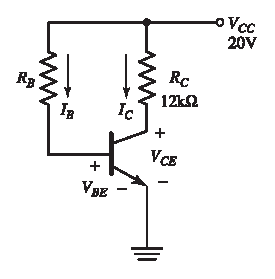
\includegraphics[scale=1.05]{chap3/S3-EE-03-IN001.eps}
\end{figure}
\end{example}

\begin{solution}
We have,
$$
V_{CC}=I_{C}R_{C}+V_{CE}
$$
When $I_{C}=0$, $V_{CE}=V_{CC}=20\text{V}$
\begin{align*}
A(V_{CE},I_{C}) &= A(20\text{V},0\text{\,mA})\\[5pt]
\text{When}\qquad I_{C}R_{C} &= V_{CC}\Rightarrow V_{CE}=0\\[5pt]
I_{C} &= \frac{V_{CC}}{R_{C}}\\[5pt]
&= \frac{20\text{V}}{12 k\Omega}\\[5pt]
&= 1.67\text{\,mA}\\[5pt]
V_{CE} &= V_{CC}-I_{C}R_{C}\\[5pt]
&= 0\text{V}\\[5pt]
B(V_{CE},I_{C}) &= B(0\text{V},1.67\text{\,mA})
\end{align*}

\eject

The following figure shows the DC load line drawn on CE output characteristics.
\begin{figure}[H]
\centering
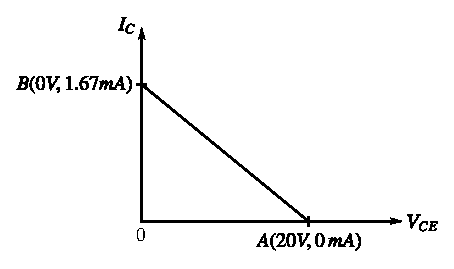
\includegraphics[scale=1.05]{chap3/sol3.1.eps}
\end{figure}
\vskip -.9cm
\end{solution}

\medskip

\begin{example}\label{exam4.2}
Repeat example \ref{exam4.1} taking $R_{C}=10 k\Omega$.
\end{example}

\begin{solution}
Change in $R_{C}$ does not affect the co-ordinates of point $A$.
$$
\therefore\qquad A(V_{CE}, I_{C})=A(20\text{V}, 0\text{\,mA})
$$
when $V_{CE}=0$,
\begin{align*}
I_{C} &= \frac{V_{CC}}{R_{C}}\\[4pt]
&= \frac{20\text{V}}{10k\Omega}\\[4pt]
&= 2\text{\,mA}\\[4pt]
\therefore\qquad B(V_{CE},I_{C}) &= B(0\text{V}, 2\text{\,mA})
\end{align*}

The dc load line drawn on CE output - characteristics is shown below.
\begin{figure}[H]
\centering
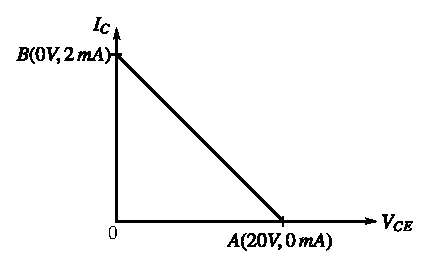
\includegraphics[scale=1.05]{chap3/sol3.2.eps}
\end{figure}
\vskip -.9cm
\end{solution}

\eject

\section[DC Bias point or $Q$ point]{DC Bias point or \boldmath$Q$ point}\label{sec4.2}

The dc bias point or quiescent point ($Q$ point)\index{Q@$Q$-point}\index{Transistor!q@$q$-point} also known as the dc operating point identifies the transistor collector current and collector-emitter voltage at a given base current, when there is no input signal at the base terminal. The intersection of DC load line with the output characteristic curve gives the co-ordinates of the $Q$ point.

\vskip .1cm

Fig.~\ref{fig4.3} shows a dc load line drawn on the CE output characteristics. 
\begin{figure}[H]
\centering
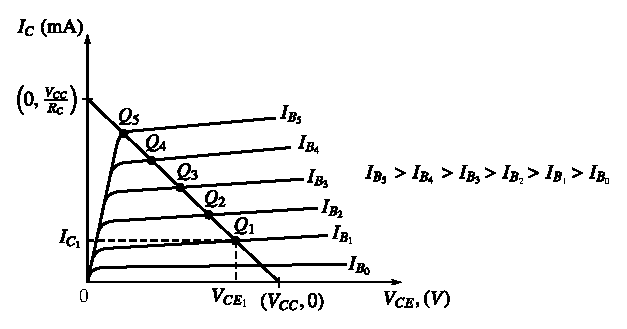
\includegraphics[scale=1.05]{chap3/fig3.3.eps}
\caption{DC bias point or $Q$ point}\label{fig4.3}
\end{figure}

The intersection of dc load line with the output characteristic curves defines the operating points $Q_{1}$, $Q_{2}$, $Q_{3}$, $Q_{4}$ and $Q_{5}$ in the active region. Note that $Q_{1}$ is near cut-off, $Q_{5}$ is near saturation and $Q_{3}$ is almost in the middle of active region (middle of dc load line). The selection of $Q$ point mainly depends upon the application.

\medskip

\heading{Meaning of \boldmath$Q_{1}$}

\vskip .15cm

If the base current level is $I_{B_{1}}$, the collector current level is $I_{C_{1}}=\beta_{\dc}I_{B_{1}}$ and the collector - emitter voltage is
$$
V_{CE_{1}}=V_{CC}-I_{C_{1}}\,R_{C}
$$

\subsection[Variation of $I_{B}$, $I_{C}$ and $V_{CE}$ with the application of input signal]{Variation of \boldmath$I_{B}$, $I_{C}$ and $V_{CE}$ with the application of input signal}\label{sec4.2.1}
\index{Transistor!biased in the active region}

Fig.~\ref{fig4.4} shows the transistor biased in the active region for the purpose of amplifying the input signal.
\begin{figure}[H]
\centering
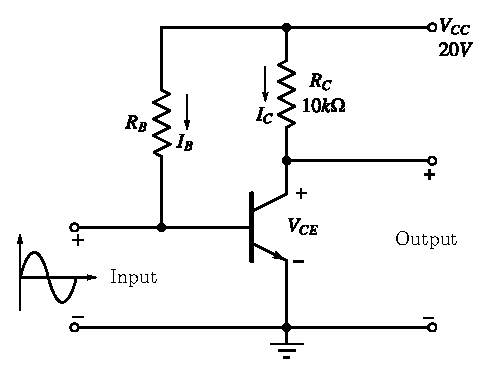
\includegraphics[scale=.9]{chap3/fig3.4.eps}
\caption{Transistor biased in active region}\label{fig4.4}
\end{figure}

The input signal to be amplified is applied between base and emitter and the amplified output is taken between collector and emitter. Hence the configuration is common-emitter.

Fig.~\ref{fig4.5} shows the dc load line drawn on the output characteristics of the transistor and the co-ordinates of the end points of the dc load line are as follows.
\begin{figure}[H]
\centering
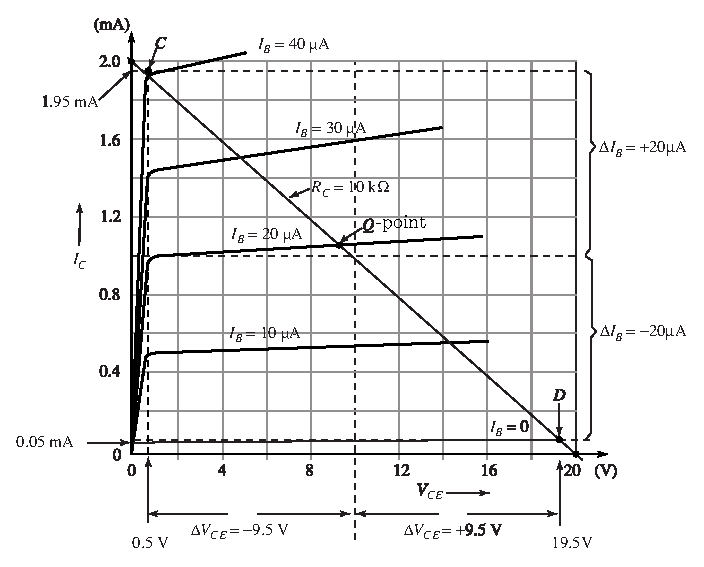
\includegraphics[scale=.9]{chap3/S3-EE-03-038.eps}
\caption{Variation of $I_{C}$ and $V_{CE}$ about $Q$ point with input signal}\label{fig4.5}
\end{figure}

\eject

~\phantom{a}

\vskip -1cm

\begin{align*}
A(V_{CE},I_{C}) &= A(20\text{V}, 0\text{\,mA})\\[4pt]
B(V_{CE},I_{C}) &= B(0\text{V},2\text{\,mA})
\end{align*}

Let us choose the $Q$ point given by the intersection of dc load line with the output characteristic curve corresponding to $I_{B}=20\,\mu\text{\,A}$. From Fig.~\ref{fig4.5},
\begin{align*}
I_{C} &= 1\text{\,mA}\\[4pt]
V_{CE} &= V_{CC}-I_{C}R_{C}=10\text{V}\\[3pt]
\therefore\qquad Q(V_{CE}, I_{C}) &= Q(10\text{V}, 1\text{mA})\text{~~ at~~ } I_{B}=20\mu\text{\,A}
\end{align*}

The application of input signal causes $I_{B}$ to vary according to the instantaneous amplitude of the signal. This causes $I_{C}$ to vary and consequently produces variation in $V_{CE}$. All these variations take place about their $Q$ point values.

When
\begin{align*}
& I_{B}\text{~~ increases from 20}\,\mu \text{A to 40}\,\mu \text{A}\\[4pt]
& I_{C}\text{~~ increases from 1\,mA to 1.95\,mA~ and}\\[4pt]
& V_{CE}\text{~~ decreases from 10\,V to 0.5\,V}
\end{align*}

Note that,
\begin{align*}
& \Delta\, I_{B} = 40\,\mu\text{\,A}-20\,\mu\text{\,A}=20\,\mu\text{\,A}\\[4pt]
& \Delta\, I_{C} = 1.95\text{\,mA}-1\text{\,mA}=0.95\text{\,mA}\\[4pt]
& \Delta\, V_{CE} = 0.5\text{\,V}-10\text{\,V}=-9.5\text{\,V}
\end{align*}
When
\begin{align*}
& I_{B} \text{~~ decreases from 20}\,\mu\,\text{A to zero}\\[4pt]
& I_{C} \text{~~ decreases from 1\,mA to 0.05\,mA \ and}\\[4pt]
& V_{CE}\text{~~ increases from 10\,V to 19.5\,V}
\end{align*}
Observe that,
\begin{align*}
& \Delta\, I_{B} = 0-20\,\mu\text{\,A}=-20\,\mu\text{\,A}\\[4pt]
& \Delta\, I_{C} = 0.05\text{\,mA}-1\text{\,mA}=-0.95\text{\,mA}\\[4pt]
& \Delta\, V_{CE} = 19.5\text{V}-10\text{V}=9.5\text{V}.
\end{align*}

\vskip .1cm

To summarise, an $I_{B}$ variation of $\pm\, 20\,\mu\text{\,A}$ results in an $I_{C}$ variation of $\pm\, 0.95\text{\,mA}$ which inturn results in a $V_{CE}$ variation of $\pm\, 9.5\text{V}$.

\eject

The actual variation in $I_{B}$, $I_{C}$ and $V_{CE}$ about their $Q$ point values depends on the amplitude of the input signal applied to the base of the transistor.


\subsection[Selection of $Q$-point]{Selection of \boldmath$Q$-point}
\index{Q@$Q$-point!selection of}

Generally the input to an amplifier is a symmetrical sine wave having equal swing of positive and negative half cycles. Therefore, when used as an amplifier the transistor output voltage $V_{CE}$ and output current $I_{C}$ must swing up and down by equal amounts from their $Q$ point values.

\vskip .1cm

In order to obtain the maximum symmetrical swing for $I_{C}$ and $V_{CE}$, the $Q$ point must be located at the centre of the dc load line as shown in Fig.~\ref{fig4.6}. The co-ordinates of the $Q$ point when located at the centre of dc load line are
$$
Q(V_{CE}, I_{C})=Q\left(\frac{V_{CC}}{2},\frac{V_{CC}}{2R_{C}}\right)
$$
\begin{figure}[H]
\centering
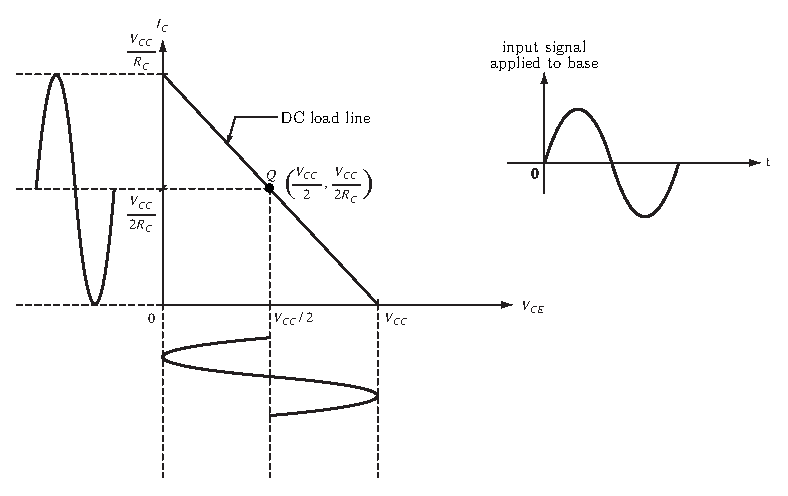
\includegraphics[scale=1.05]{chap3/S3-EE-03-039.eps}
\bigskip
\caption{Maximum swings of $I_{C}$ and $V_{CE}$ with the $Q$ point at the centre of DC load line}\label{fig4.6}
\end{figure}

\eject

From Fig.~\ref{fig4.6}, we make the following observations. 

Maximum upward swing of $I_{C}$~:
$$
\frac{V_{CC}}{R_{C}}-\frac{V_{CC}}{2R_{C}}=\frac{V_{CC}}{2R_{C}}
$$
Maximum downward swing of $I_{C}$~:
$$
0-\frac{V_{CC}}{2R_{C}}=-\frac{V_{CC}}{2R_{C}}
$$
$\Rightarrow$~ Maximum variation of $I_{C}$ about $Q$ point~:
$$
\pm \ \frac{V_{CC}}{2R_{C}}
$$
Maximum upward swing of $V_{CE}$~:
$$
V_{CC}-\frac{V_{CC}}{2}=\frac{V_{CC}}{2}
$$
Maximum downward swing of $V_{CE}$~:
$$
0-\frac{V_{CC}}{2}=-\frac{V_{CC}}{2}
$$
$\Rightarrow$~ Maximum variation of $V_{CE}$ about $Q$ point
$$
\pm \ \frac{V_{CC}}{2}
$$
Observe that the swing in $I_{C}$ and $V_{CE}$ is maximum and symmetrical about their $Q$ point values.

\vskip .1cm

If the $Q$ point is located near the lower end of dc load line (near cut-off point), the positive peak of output voltage (or the negative peak of output current) may be clipped off as shown in Fig.~\ref{fig4.7}. This is due to the fact that, the allowable swing for increasing part of output voltage (or decreasing part of output current) is small. Note that the swing in $I_{C}$ and $V_{CE}$ is unsymmetrical.

\vskip .1cm

If the $Q$ point is located near the upper end of dc load line (near saturation point), the negative peak of output voltage (or positive peak of output current) may be clipped off as shown in Fig.~\ref{fig4.8}. In this case the allowable swing for decreasing part of output voltage (or increasing part of output current) is small. Also the swing in $I_{C}$ and $V_{CE}$ is unsymmetrical. Clipping of the output wave form results in distorted output.
\begin{figure}[H]
\centering
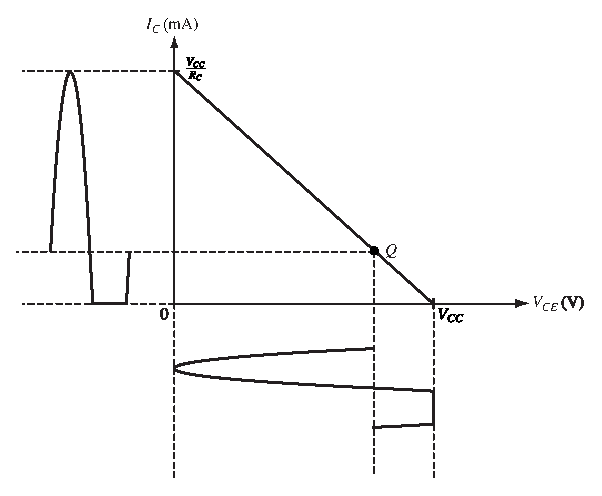
\includegraphics{chap3/S3-EE-03-040.eps}
\caption{Clipping of output voltage and current waveforms when the $Q$ point is near cut-off}\label{fig4.7}
\end{figure}

\begin{figure}[H]
\centering
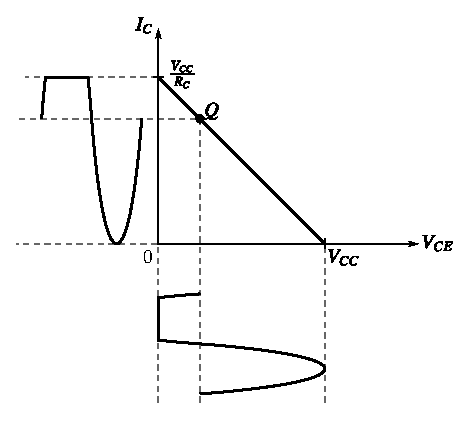
\includegraphics{chap3/fig3.8.eps}
\caption{Clipping of output voltage and current wave forms when the $Q$ point is near saturation}\label{fig4.8}
\end{figure}

\heading{Conclusion~:}

{\em In order to obtain maximum undistorted swing of output voltage and current in an amplifier the $Q$ point must be located at the centre of dc load line.}

\section{Biasing circuits}\label{sec4.3}

Biasing circuits\index{Biasing circuits}\index{Transistor!biasing circuits} employ a resistive network and a dc power supply to establish the required dc currents and voltages in the transistor circuit. A variety of biasing circuits exist. Among these, base bias is simplest and voltage divider bias is the best as mentioned earlier. Base bias circuit is more common in transistor switching circuits. Voltage divider bias is predominantly used in amplifier circuits.

\subsection{Requirements of a Biasing circuit}\label{sec4.3.1}
\index{Biasing circuits!requirements of}

A biasing circuit used to bias BJT must fulfil the following requirements:
\begin{enumerate}
\item Establish proper voltages and currents so that the transistor operates in the appropriate region of its characteristics. In the application of transistor as an amplifier, the biasing circuit must fix the $Q$ point in the middle of active region so that a large symmetrical swing of the output voltage is allowed with no distortion.

\item Ensure almost constant collector current, $I_{C}$, despite temperature variations.

\item Make the operating point independent of transistor parameters so that replacement of transistor by another of same type in the circuit does not shift the $Q$ point.
\end{enumerate}

Summarizing, the function of a biasing circuit is not only to establish the appropriate $Q$ point but also make it independent of temperature and device parameters.

\section{Base bias or Fixed current Bias}\label{sec4.4}
\index{Biasing circuits!base bias}\index{Transistor!base bias}
\index{Fixed current Bias}

Fig.~\ref{fig4.9} shows the base bias\index{Base bias} circuit.
The bias current $I_{B}$ for the transistor is derived from the dc supply $V_{CC}$ through the resistor $R_{B}$. Applying Kirchhoff's Voltage Law to the base-emitter circuit we have
\begin{align}
V_{CC} &= I_{B}R_{B}+V_{BE}\notag\\[4pt]
I_{B} &= \frac{V_{CC}-V_{BE}}{R_{B}}\label{eq4.11} 
\end{align}
$V_{BE}$ is taken as 0.7V for a Silicon transistor and as 0.3V for a Germanium transistor. Usually $V_{CC}\gg V_{BE}$.

\eject

Therefore \ $V_{CC}-V_{BE}\simeq V_{CC}$. Now, from Eqn.~\eqref{eq4.11} we have
\begin{equation}
I_{B}\simeq \frac{V_{CC}}{R_{B}}\label{eq4.12}
\end{equation}

\begin{figure}[H]
\centering
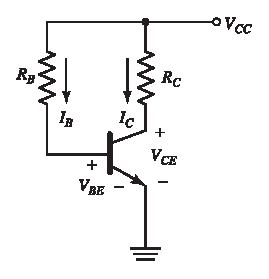
\includegraphics{chap3/S3-EE-03-041.eps}
\caption{Base bias circuit}\label{fig4.9}
\end{figure}

Since $V_{CC}$ and $R_{B}$ are constant quantities, $I_{B}$ is a constant quantity. Hence base bias is also called as fixed current bias.\index{Transistor!fixed current bias}\index{Biasing circuits!fixed current bias}

The collector current is calculated as
\begin{equation}
I_{C}=h_{FE}I_{B}\label{eq4.13}
\end{equation}

The collector to emitter voltage $V_{CE}$ is obtained by applying Kirchhoff's Voltage Law to the collector emitter circuit.
\begin{align}
V_{CC} &= I_{C}R_{C}+V_{CE}\notag\\[3pt]
V_{CE} &= V_{CC}-I_{C}R_{C}\label{eq4.14}
\end{align}

Using Eqns.~\eqref{eq4.11}, \eqref{eq4.13} and \eqref{eq4.14} we can find $I_{B}$, $I_{C}$ and $V_{CE}$ when $V_{CC}$, $R_{C}$, $R_{B}$ and $h_{FE}$ are known.

\begin{example}\label{exam4.3}
For the base bias circuit shown in Fig.~\ref{fig4.9}, find $I_{B}$, $I_{C}$ and $V_{CE}$ if $R_{C}=2.2 k\Omega$, $R_{B}=470 k\Omega$, $V_{CC}=18\text{V}$, $h_{FE}=100$, $V_{BE}=0.7\text{V}$. Draw the DC load line and indicate the $Q$ point.
\end{example}

\begin{solution}
Given, $R_{C}=2.2\, k\,\Omega$, $R_{B}=470\, k\,\Omega$, $V_{CC}=18\text{V}$, $V_{BE}=0.7\text{V}$, $h_{FE}=100$
\begin{align*}
I_{B} &= \frac{V_{CC}-V_{BE}}{R_{B}}\\[2pt]
&= \frac{18\text{V}-0.7\text{V}}{470\,k\,\Omega}\\[2pt]
&= 36.81\mu\text{A}\\[2pt]
I_{C} &= h_{FE}I_{B}\\[2pt]
&= 100\times 36.81 \mu\text{A}\\[2pt]
&= 3.68\text{\,mA}\\[2pt]
V_{CE} &= V_{CC}-I_{C}R_{C}\\[2pt]
&= 18\text{V}-(3.68\text{\,mA}\times 2.2 k\Omega)\\[2pt]
&= 9.9\text{V}
\end{align*}
Co-ordinates of $Q$ point are $Q(V_{CE},I_{C})=Q(9.9\text{V},3.68\text{\,mA})$. The $dc$ load line is shown in the following Figure.
\end{solution}

\begin{figure}[H]
\centering
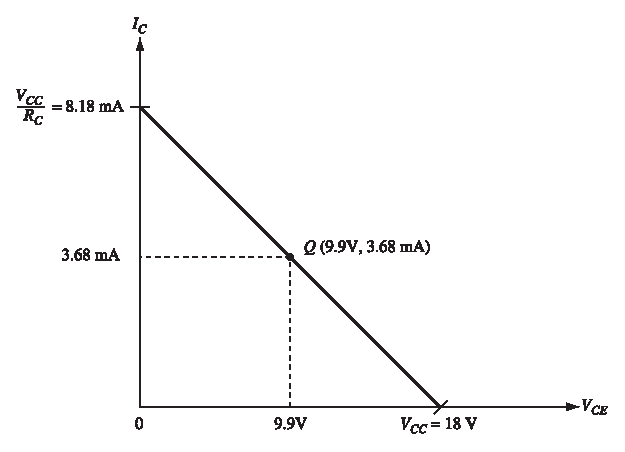
\includegraphics{chap3/S3-EE-03-IN003.eps}
\end{figure}
\noindent
{\bf Note:}
\begin{itemize}
\item[(1)] $1\text{\,mA}\times 1 k\Omega=10^{-3}\text{A}\times 10^{3}\Omega=1\text{V}$

\item[(2)] If $V_{BE}$ is not specified we can assume either Silicon or Germanium transistor. $V_{BE}$ is $0.3\text{V}$ for gemanium transistor and 0.7V for Silicon transistor.
\end{itemize}

\begin{example}\label{exam4.4}
For the base-bias circuit shown in Fig.~\ref{fig4.9}, $V_{CC}=18\text{V}$, $R_{C}=2.2\, k\Omega$, $R_{B}=470\, k\Omega$, $V_{BE}=0.7\text{V}$. Find the levels of $I_{C}$ and $V_{CE}$ when $h_{FE(\min)}=50$ and $h_{FE(\max)}=200$. Draw the dc line and indicate the $Q$ points. Also find maximum and minimum levels of $I_{C}$ and $V_{CE}$.
\end{example}

\eject

\begin{solution}
\begin{description}
\item[{\bf Case 1:}] When \ $h_{FE}=h_{FE(\min)}=50$
\begin{align*}
I_{B} &= \frac{V_{CC}-V_{BE}}{R_{B}}\\[3pt]
&= \frac{18\text{V}-0.7\text{V}}{470 k\Omega}=36.81\mu \text{A}\\[3pt]
I_{C} &= h_{FE(\min)}\,I_{B}\\[3pt]
&= 50\times 36.81\mu\text{A}=1.84\text{\,mA}\\[3pt]
V_{CE} &= V_{CC}-I_{C}R_{C}\\[3pt]
&= 18\text{V}-(1.84\text{\,mA}\times 2.2 k\Omega)=13.95\text{V}\\[3pt]
Q_{1}(V_{CE},I_{C}) &= Q_{1}(13.95\text{V},1.84\text{\,mA})
\end{align*}

\item[{\bf Case 2:}] When \ $h_{FE}=h_{FE(\max)} =200$
\begin{align*}
I_{B}&= \frac{V_{CC}-V_{BE}}{R_{B}}\\[3pt]
&= \frac{18\text{V}-0.7\text{V}}{470 k\Omega}\\[3pt]
&= 36.81\mu\text{A}
\end{align*}
Note that $I_{B}$ is unaffected by $h_{FE}$
\begin{align*}
I_{C} &= h_{FE(\max)}\,I_{B}\\[3pt]
&= 200\times 36.81\mu\text{A}\\[3pt]
&= 7.36\text{\,mA}\\[3pt]
V_{CE} &= V_{CC}-I_{C}R_{C}\\[3pt]
&= 18\text{V}-(7.36\text{\,mA}\times 2.2 k\Omega)\\[3pt]
&= 1.81\text{V}\\[3pt]
Q_{2}(V_{CE},I_{C}) &= Q_{2}(1.81\text{V}, \ 7.36\text{\,mA})
\end{align*}

Maximum and minimum levels of $I_{C}$ and $V_{CE}$~:

{\em When $h_{FE}=h_{FE(\min)}=50$}
\begin{align*}
V_{CE(\max)} &= 13.95\text{V}\\
I_{C(\min)} &= 1.84\text{\,mA}
\end{align*}

\vfill\eject

{\em When $h_{FE}=h_{FE(\max)}=200$}
\begin{align*}
V_{CE(\min)} &= 1.81\text{V}\\[3pt]
I_{C(\max)} &= 7.36\text{\,mA}
\end{align*}
\end{description}
\vskip -.5cm
\begin{figure}[H]
\centering
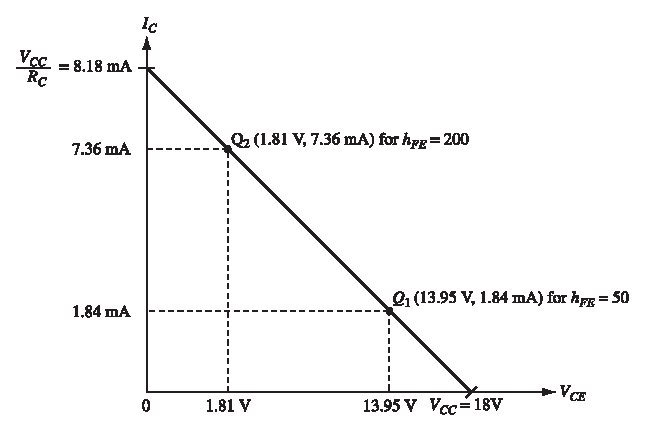
\includegraphics[scale=.9]{chap3/S3-EE-03-IN004.eps}
\end{figure}
\vskip -.9cm
\end{solution}

\smallskip

\noindent
{\bf Note:}~
This problem investigates the effect of $h_{FE}$ variation on the stability of $Q$ point in base bias circuit, note that when $h_{FE}$ changes from 50 to 200, the $Q$ point shifts drastically. Hence the base bias circuit has poor $Q$ point stability.

\smallskip
\begin{example}\label{exam4.5}
In the circuit shown, a Silicon transistor with $\beta_{\dc}=100$ is used. Find $I_{C}$ and $V_{CE}$. Draw the DC load line on the output characteristics and indicate the $Q$ point. Assume $V_{BE}=0.7\text{V}$.
\begin{figure}[H]
\centering
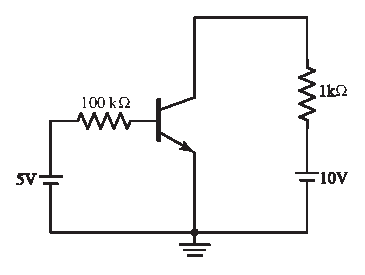
\includegraphics{chap3/S3-EE-03-IN005.eps}
\end{figure}
\end{example}

\eject

\begin{solution}
Let us redraw the given circuit by marking the various voltages and currents as shown below.
\begin{figure}[H]
\centering
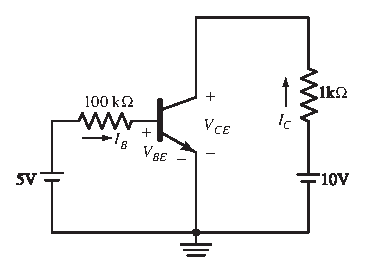
\includegraphics[scale=1.1]{chap3/S3-EE-03-IN006.eps}
\end{figure}

Applying Kirchhoff's Voltage Law to base-emitter circuit.
\begin{align*}
5\text{V}-I_{B}(100\,k\Omega)-V_{BE} &=0\\[4pt]
I_{B} &= \frac{5\text{V}-V_{BE}}{100\, k\Omega}\\[4pt]
&= \frac{5\text{V}-0.7\text{V}}{100\, k\Omega}\\[4pt]
&= 0.043\text{\,mA}\text{~~ or~~ } 43\mu\text{\,A}\\[4pt]
I_{C} &= h_{FE}I_{B}\\[4pt]
h_{FE} &= \beta_{\dc} = 100\\[4pt]
I_{C} &= (100)(0.043\text{\,mA})\\[4pt]
&= 4.3\text{\,mA} 
\end{align*}

Applying Kirchhoff's Voltage Law to the collector-emitter circuit we have,
\begin{align*}
10\text{V}-I_{C}(1 k\Omega)-V_{CE} &= 0\\[4pt]
V_{CE} &= 10\text{V}-(4.3\text{\,mA})(1 k\Omega)\\[4pt]
V_{CE} &= 5.7\text{V}\\[4pt]
Q(V_{CE},I_{C}) &= Q(5.7\text{V}, 4.3\text{\,mA})
\end{align*}
\begin{figure}[H]
\centering
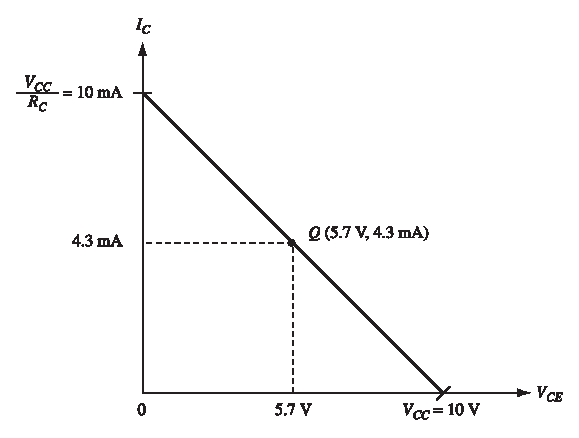
\includegraphics{chap3/S3-EE-03-IN007.eps}
\end{figure}
\vskip -1cm
\end{solution}

\begin{example}\label{exam4.6}
In the circuit shown below a Silicon transistor with $\beta=50$ is used. Find $I_{C}$ and $V_{CE}$. Draw the DC load line on the output characteristics and indicate the $Q$ point. Take $V_{BE}=0.7\text{V}$.
\begin{figure}[H]
\centering
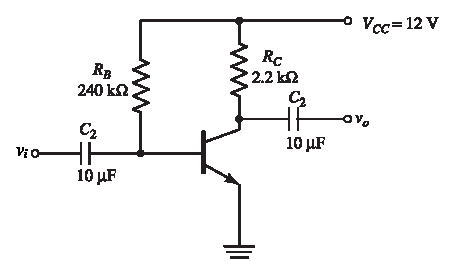
\includegraphics{chap3/S3-EE-03-IN008.eps}
\end{figure}
\end{example}

\begin{solution}
Since we are carrying out dc analysis, all capacitors can be treated as open circuits. Let us redraw the circuit with various currents and voltages indicated.
\begin{figure}[H]
\centering
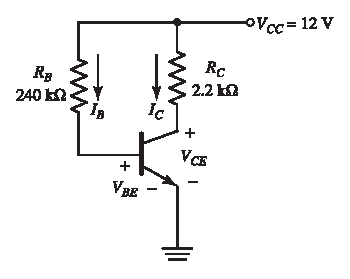
\includegraphics{chap3/S3-EE-03-IN009.eps}
\end{figure}

\eject

~\phantom{a}
\vskip -1cm

\begin{align*}
I_{B} &= \frac{V_{CC}-V_{BE}}{R_{B}}\\[5pt]
&= \frac{12\text{V}-0.7\text{V}}{240\, k\Omega}\\[5pt]
&= 0.047\text{\,mA}\text{~~ or~~ } 47\,\mu\text{A}\\[5pt]
I_{C} &= h_{FE}I_{B}\\[5pt]
\beta &= h_{FE}=50\\[5pt]
I_{C} &= (50)(0.047\text{\,mA})\\[5pt]
&= 2.35\text{\,mA}\\[5pt]
V_{CE} &= V_{CC}-I_{C}R_{C}\\[5pt]
&= 12\text{V}-(2.35\text{\,mA})(2.2 k\Omega)\\[5pt]
&= 6.83\text{V}\\[5pt]
Q(V_{CE},I_{C}) &= Q(6.83\text{V},2.35\text{\,mA})
\end{align*}
The $dc$ load line is shown in the following figure.
\begin{figure}[H]
\centering
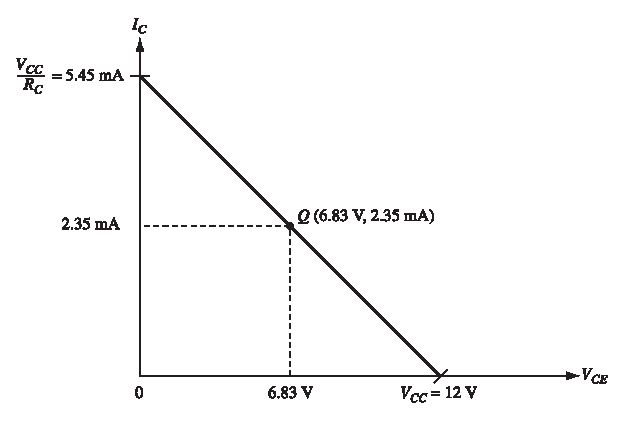
\includegraphics[scale=1.07]{chap3/S3-EE-03-IN010.eps}
\end{figure}
\vskip -1cm
\end{solution}

\eject

\begin{example}\label{exam4.7}
For the circuit shown below draw the DC load line and mark the dc operating point on it. Assume $\beta=100$ and neglect $V_{BE}$.
\begin{figure}[H]
\centering
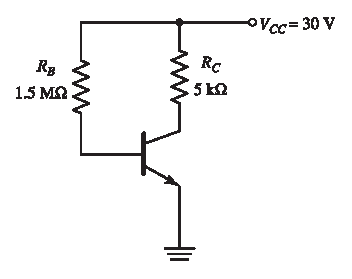
\includegraphics{chap3/S3-EE-03-IN011.eps}
\end{figure}
\end{example}

\begin{solution}
Let us redraw the given circuit with all voltages and currents marked.
\begin{figure}[H]
\centering
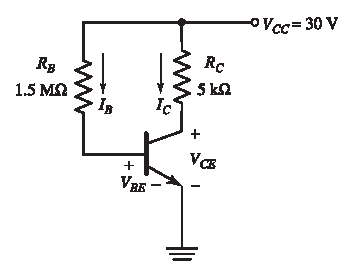
\includegraphics{chap3/S3-EE-03-IN012.eps}
\end{figure}
\begin{align*}
I_{B} &= \frac{V_{CC}-V_{BE}}{R_{B}}=\frac{V_{CC}}{R_{B}}\quad\text{(Neglecting $V_{BE}$)}\\[4pt]
&= \frac{30\text{V}}{1.5\, M\Omega}=\frac{30\text{V}}{1500\,k\Omega}=0.02\text{\,mA}\\[4pt]
I_{C} &= h_{FE}I_{B}\\[4pt]
\beta &= h_{FE}=100\\[4pt]
I_{C} &= (100)(0.02\text{\,mA})=2\text{\,mA}\\[4pt]
V_{CE} &= V_{CC}-I_{C}R_{C}\\[4pt]
&= 30\text{V}-(2\text{\,mA})(5\,k\Omega)=20\text{V}\\[4pt]
Q(V_{CE},I_{C}) &= Q(20\text{V}, 2\text{\,mA})
\end{align*}
The $dc$ load line is shown in the following figure.

\vfill\eject

\begin{figure}[H]
\centering
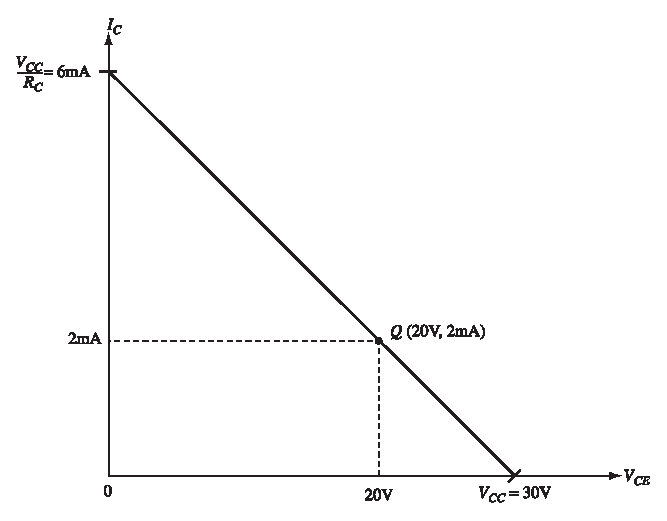
\includegraphics[scale=.9]{chap3/S3-EE-03-IN013.eps}
\end{figure}
\vskip -.9cm
\end{solution}

\begin{example}\label{exam4.8}
A base bias circuit has $V_{CC}=24\text{V}$, $R_{B}=390\,k\Omega$, $R_{C}=3.3\,k\Omega$ and $V_{CE}=10\text{V}$. Calculate the transistor $h_{FE}$ value. Determine the new $V_{CE}$ level when a new transistor is substituted with $h_{FE}=100$.
\end{example}

\begin{solution}
The base bias circuit with circuit paramter values is shown below.
\begin{figure}[H]
\centering
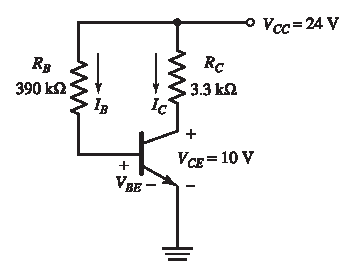
\includegraphics{chap3/S3-EE-03-IN014.eps}
\end{figure}
\begin{align*}
V_{CC} &= I_{C}R_{C}+V_{CE}\\[7pt]
I_{C} &= \frac{V_{CC}-V_{CE}}{R_{C}}
= \frac{24\text{V}-10\text{V}}{3.3\, k\Omega}
= 4.24\text{\,mA}\\[7pt]
I_{B} &= \frac{V_{CC}-V_{BE}}{R_{B}}
\end{align*}

\eject

\noindent
Assuming Silicon transistor for which $V_{BE}=0.7\text{V}$
\begin{align*}
I_{B} &= \frac{24\text{V}-0.7\text{V}}{390 k\Omega}=0.0597\text{\,mA}\\[4pt]
I_{C} &= h_{FE}I_{B}\\[4pt]
\Longrightarrow \ h_{FE} &= \frac{I_{C}}{I_{B}}\\[4pt]
&= \frac{4.24\text{\,mA}}{0.0597\text{\,mA}}\\[4pt]
&= 71
\end{align*}
To find $V_{CE}$ when $h_{FE}=100$
\begin{align*}
I_{B} &= \frac{V_{CC}-V_{BE}}{R_{B}}=0.0597\text{\,mA}\quad \text{[same as before]}\\[4pt]
I_{C} &= h_{FE}I_{B}=100(0.0597\text{\,mA})\\[4pt]
&= 5.97\text{\,mA}\\[4pt]
V_{CE} &= V_{CC}-I_{C}R_{C}\\[4pt]
&= 24\text{V}-(5.97\text{\,mA})(3.5 k\Omega)\\[4pt]
&= 4.29\text{V}.
\end{align*}
\vskip -.7cm
\end{solution}

\smallskip

\begin{example}\label{exam4.9}
For the circuit shown, determine the $Q$ point and estimate the maximum symmetrical output voltage swing. Take $h_{FE}=100$ and $V_{BE}=0.7\text{V}$.
\begin{figure}[H]
\centering
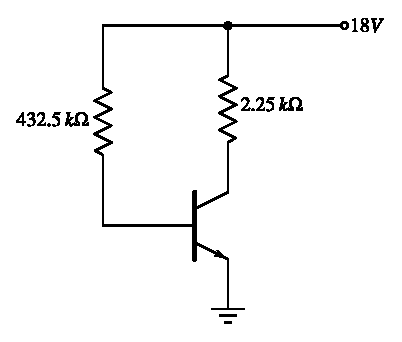
\includegraphics{chap3/exp3.9.eps}
\end{figure}
\end{example}

\eject

\begin{solution}
\begin{align*}
I_{B} &= \frac{V_{CC}-V_{BE}}{R_{B}}\\[4pt]
&= \frac{18\text{V}-0.7\text{V}}{432.5 k\Omega}\\[4pt]
&= 40\text{\,mA}\\[7pt]
I_{C} &= h_{FE}I_{B}\\[4pt]
&= 100 (40\text{\,mA})\\[4pt]
&= 4\text{\,mA}\\[7pt]
V_{CE} &= V_{CC}-I_{C}R_{C}\\[4pt]
&= 18\text{V}-(4\text{\,mA})(2.25 k\Omega)\\[4pt]
&= 9\text{V}\\[4pt]
\frac{V_{CC}}{R_{C}} &= \frac{18\text{V}}{2.25 k\Omega}=8\text{\,mA}
\end{align*}
The load line drawn on output characteristics is shown below
\begin{figure}[H]
\centering
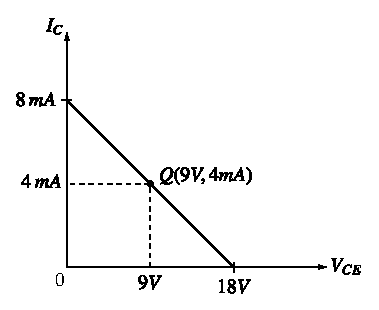
\includegraphics{chap3/sol3.9.eps}
\end{figure}

Since the $Q$ point is at the centre of dc load line, the output voltage swing is symmetrical and maximum. Therefore maximum symmetrical output voltage swing is
\begin{align*}
&= (0-9\text{V})\quad\text{or}\quad (18\text{V}-9\text{V})\\[4pt]
&= -\,9\text{V}\quad\text{or}\quad + 9\text{V}\\[4pt]
&= \pm\, 9\text{V}.
\end{align*}
\vskip -.7cm
\end{solution}

\eject

\begin{example}\label{exam4.10}
For the circuit shown find the $Q$ point and estimate the maximum symmetrical output voltage swing.

\vskip .1cm

For the transistor $h_{FE}=100$.
\begin{figure}[H]
\centering
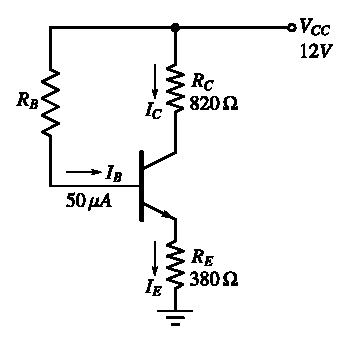
\includegraphics[scale=1.05]{chap3/exp3.10.eps}
\end{figure}
\end{example}

\begin{solution}
\begin{align*}
I_{B} &= 50\,\mu\text{\,A}\\[5pt]
I_{C} &= h_{FE}I_{B}\\[5pt]
&= (100)(50\,\mu\text{A})\\[5pt]
&= 5\text{\,mA}\\[8pt]
I_{E} &= I_{B}+I_{C}\\[5pt]
&= 50\,\mu\text{A}+5\text{\,mA}\\[5pt]
&\approx 5\text{\,mA}\\[8pt]
V_{CC} &= I_{C}R_{C}+V_{CE}+I_{E}R_{E}\tag{A}\\[5pt]
V_{CE} &= V_{CC}-I_{C}R_{C}-I_{C}R_{E}\\[5pt]
&= 12\text{V}-(5\text{\,mA})(820 \Omega)-(5\text{\,mA})(380 \Omega)\\[5pt]
&= 6\text{V}\\[5pt]
Q(V_{CE},I_{C}) &= Q(6\text{V}, 5\text{\,mA})
\end{align*}

\eject

\heading{When \boldmath$I_{C}=0$}

\vskip .1cm

From Eqn.~(A)
\begin{align*}
V_{CE} &\approx V_{CC}\quad \text{[since $I_{E}\approx 0$]}\\[4pt]
&= 12\text{V}\\[4pt]
A(V_{CE}, I_{C}) &= A(V_{CC},0)=A(12\text{V},0\text{\,mA})
\end{align*}

\vskip .1cm
\heading{When \boldmath$V_{CE}=0$}

\vskip .1cm
Again from Eqn.~(A)
\begin{align*}
V_{CC} &= I_{C}R_{C}+I_{E}R_{E}\\[4pt]
\text{or}\qquad I_{C} &\approx \frac{V_{CC}}{R_{C}+R_{E}}\\[4pt]
I_{C} &= \frac{12\text{V}}{820\Omega +380 \Omega}\\[4pt]
&= 10\text{\,mA}\\[4pt]
B(V_{CE},I_{C}) &= B(0\text{V}, 10\text{\,mA})
\end{align*}
The load line drawn on output characteristics is shown below.
\begin{figure}[H]
\centering
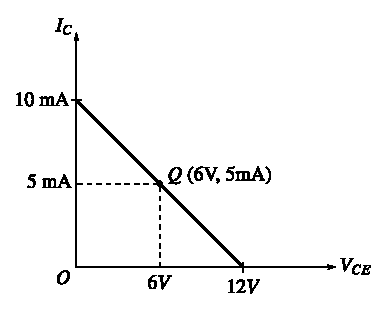
\includegraphics[scale=1.05]{chap3/sol3.10.eps}
\end{figure}

From the figure, maximum symmetrical output voltage swing
\begin{align*}
&= (0-6\text{V})\quad\text{or}\quad (12\text{V}-6\text{V})\\[4pt]
&= -6\text{V}\quad\text{or}\quad +6\text{V}\\[4pt]
&= \pm\, 6\text{V}
\end{align*}
\vskip -.7cm
\end{solution}

\eject

\section{Design of Base-bias circuit}\label{sec4.5}
\index{Base bias!design of}

The base bias circuit is shown in Fig.~\ref{fig4.10}.
\begin{figure}[H]
\centering
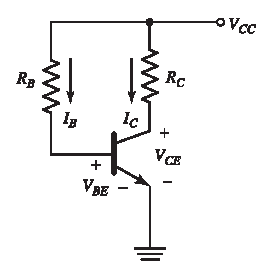
\includegraphics[scale=1.25]{chap3/S3-EE-03-042.eps}
\caption{Base-bias circuit}\label{fig4.10}
\end{figure}

The values of $V_{CC}$, $V_{CE}$, $V_{BE}$, $I_{C}$ and $h_{FE}$ will be given. The design steps are as follows:
\begin{itemize}
\item First calculate $R_{C}$ using the relation
\begin{equation}
R_{C}=\frac{V_{CC}-V_{CE}}{I_{C}}\label{eq4.15}
\end{equation}

\item Then calculate $I_{B}$ using the relation
\begin{equation}
I_{B}=\frac{I_{C}}{h_{FE}}\label{eq4.16}
\end{equation}

\item Finally calculate $R_{B}$ using the relation
\begin{equation}
R_{B}=\frac{V_{CC}-V_{BE}}{I_{B}}\label{eq4.17}
\end{equation}
\end{itemize}

\eject

\begin{example}\label{exam4.11}
Design a base bias circuit to have $V_{CE}=5\text{V}$ and $I_{C}=5\text{\,mA}$. The supply voltage is $15\text{V}$ and the transistor has $h_{FE}=100$.
\end{example}

\begin{solution}
Given,
\begin{align*}
V_{CE} &= 5\text{V},\quad I_{C}=5\text{\,mA}\\[5pt]
V_{CC} &= 15\text{V},\quad h_{FE}=100\\[5pt]
R_{C} &= \frac{V_{CC}-V_{CE}}{I_{C}}\\[5pt]
&= \frac{15\text{V}-5\text{V}}{5\text{\,mA}}\\[5pt]
&= 2\,k\Omega\\[5pt]
I_{B} &= \frac{I_{C}}{h_{FE}}\\[5pt]
&= \frac{5\text{\,mA}}{100}\\[5pt]
&= 0.05\text{\,mA}\\[5pt]
R_{B} &= \frac{V_{CC}-V_{BE}}{I_{B}}
\end{align*}
Assume a Silicon transistor for which $V_{BE}=0.7\text{V}$
$$
\therefore\quad R_{B}=\frac{15\text{V}-0.7\text{V}}{0.05\text{\,mA}}=286 k\Omega
$$ 
The base bias circuit with component values is shown below.
\begin{figure}[H]
\centering
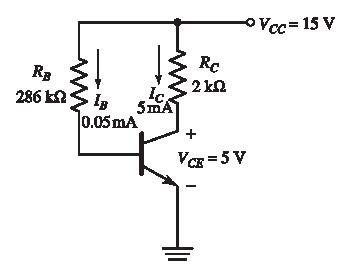
\includegraphics[scale=1.1]{chap3/S3-EE-03-IN015.eps}
\end{figure}
\vskip -.7cm
\end{solution}

\vfill\eject

\begin{example}\label{exam4.12}
A base bias circuit with $V_{CC}=18\text{V}$ uses a transistor with $V_{BE}=0.7\text{V}$. The circuit is to have $V_{CE}=9\text{V}$ and $I_{C}=2\text{\,mA}$. Plot the $Q$ point, draw the $DC$ load line and determine the required value of $R_{C}$. 
\end{example}

\begin{solution}
Given,
\begin{align*}
V_{CC} &= 18\text{V},\quad V_{BE}=0.7\text{V}\\[4pt]
V_{CE} &= 9\text{V},\quad I_{C}=2\text{\,mA}\\[4pt]
R_{C} &= \frac{V_{CC}-V_{CE}}{I_{C}}= \frac{18\text{V}-9\text{V}}{2\text{\,mA}}\\[4pt]
&= 4.5 k\Omega
\end{align*}
The load line is shown in the following figure.
\begin{figure}[H]
\centering
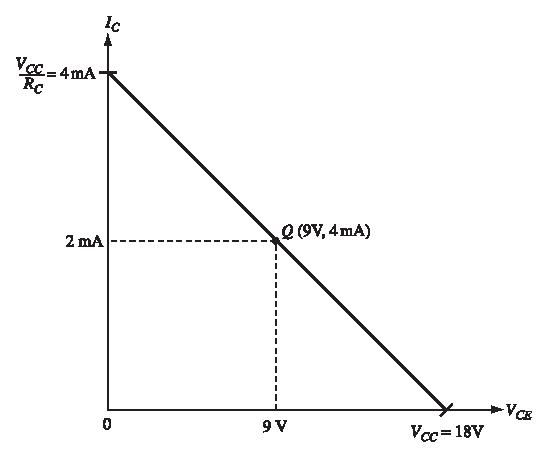
\includegraphics{chap3/S3-EE-03-IN016.eps}
\end{figure}
\vskip -.9cm
\end{solution}

\begin{example}\label{exam4.13}
A base bias circuit has $V_{CC}=20\text{V}$, $R_{C}=6.8\,k\Omega$ and the transistor has $h_{FE}=120$. Calculate the required base resistance value to give $V_{CE}=5\text{V}$.
\end{example}

\begin{solution}
Given,
\begin{align*}
V_{CC} &= 20\text{V},\quad V_{CE}=5\text{V}\\[4pt]
R_{C} &= 6.8\,k\Omega,\quad h_{FE}=120\\[4pt]
I_{C} &= \frac{V_{CC}-V_{CE}}{R_{C}}\\[4pt]
&= \frac{20\text{V}-5\text{V}}{6.8\,k\Omega}=2.21\text{\,mA}\\[4pt]
I_{B} &= \frac{I_{C}}{h_{FE}}\\[4pt]
&= \frac{2.21\text{\,mA}}{120}\\[4pt]
&= 0.0184\text{\,mA}\\[4pt]
R_{B} &= \frac{V_{CC}-V_{BE}}{I_{B}}
\end{align*}
Assume a Silicon transistor for which $V_{BE}=0.7\text{V}$
\begin{align*}
R_{B} &= \frac{20\text{V}-0.7\text{V}}{0.0184\text{\,mA}}\\[4pt]
&= 1048.91 k\Omega
\end{align*}
\vskip -.7cm
\end{solution}

\section{Voltage divider bias circuit}\label{sec4.6}
\index{Biasing circuits!voltage divider bias}\index{Transistor!voltage divider bias}

Voltage divider bias\index{Voltage divider bias} also known as emitter current bias\index{Emitter current bias} or universal bias\index{Universal bias} gives the most stable operating point when compared to all other biasing circuits. Fig.~\ref{fig4.11} shows the circuit of voltage divider bias.
\begin{figure}[H]
\centering
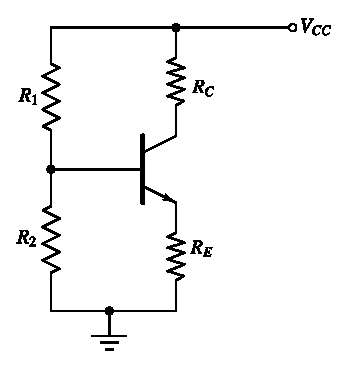
\includegraphics{chap3/fig3.11.eps}
\caption{Voltage divider bias circuit}\label{fig4.11}
\end{figure}

The dc supply voltage is divided using the voltage divider network consisting of $R_{1}$ and $R_{2}$. The voltage across $R_{2}$ is applied between base and ground to provide the required forward bias on the base-emitter juntion.

The emitter resistance $R_{E}$ is used to provide the stability of $Q$ point. $R_{C}$ along with $R_{E}$ decides the collector current level in the circuit.

\section{Analysis of voltage divider bias circuit}\label{sec4.7}
\index{Voltage divider bias!analysis of}

Voltage divider bias circuit can be analysed in the following two ways, depending upon the circuit condition.
\begin{itemize}
\item[(a)] Approximate analysis.

\item[(b)] Accurate or exact analysis.
\end{itemize}

\subsection{Approximate analysis of voltage divider bias circuit}\label{sec4.7.1}


Fig.~\ref{fig4.12} shows the voltage divider bias circuit with all currents and voltages indicated.
\begin{figure}[H]
\centering
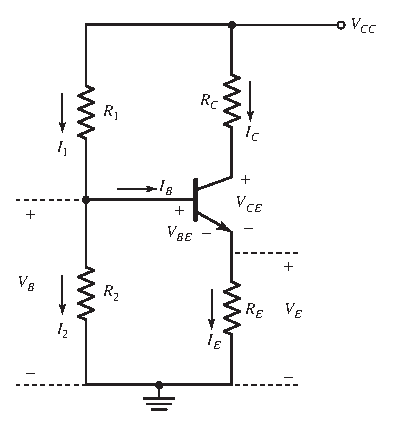
\includegraphics[scale=1.05]{chap3/S3-EE-03-045.eps}
\caption{Voltage divider bias circuit}\label{fig4.12}
\end{figure}

Applying KCL at the base node, we have
\begin{equation}
I_{1}=I_{2}+I_{B}\label{eq4.18}
\end{equation}

Approximate analysis can be used, if
\begin{equation}
I_{2} \gg I_{B}\label{eq4.19}
\end{equation}
Under this condition, 
\begin{equation}
I_{1}\approx I_{2}\label{eq4.20}
\end{equation}

For the voltage divider network
$$
V_{CC}=I_{1}R_{1}+I_{2}R_{2}
$$

Since, $I_{1}\approx I_{2}$, we have
\begin{equation}
I_{1}=I_{2}=\frac{V_{CC}}{R_{1}+R_{2}}\label{eq4.21}
\end{equation}

Voltage across $R_{2}$ is, $V_{B}=I_{2}\,R_{2}$
\begin{equation}
V_{B}=\frac{V_{CC}R_{2}}{R_{1}+R_{2}}\label{eq4.22}
\end{equation}

Note that $V_{B}$ is a constant quantity
\begin{align}
& V_{B}=V_{BE}+V_{E}\notag\\[3pt]
& V_{E}=V_{B}-V_{BE}\label{eq4.23}
\end{align}

But $V_{E}=I_{E}R_{E}$. Using this relation in Eqn.~\eqref{eq4.23}
\begin{align}
I_{E}R_{E} &= V_{B}-V_{BE}\notag\\[3pt]
I_{E} &= \frac{V_{B}-V_{BE}}{R_{E}}=\frac{V_{E}}{R_{E}}\label{eq4.24}
\end{align}
$I_{E}=I_{B}+I_{C}\simeq I_{C}$, since base current is small. Since $V_{B}$ is a constant quantity, $I_{C}$ and $I_{E}$ are held at constant level.

Applying Kirchhoff's Voltage Law to the collector emitter circuit we have
$$
V_{CC}=I_{C}R_{C}+V_{CE}+I_{E}R_{E}
$$
Since $I_{E}\simeq I_{C}$, we can write
\begin{equation}
V_{CE}=V_{CC}-I_{C}\,(R_{C}+R_{E})\label{eq4.25}
\end{equation}

Clearly, with $I_{C}$ and $I_{E}$ constant, the transistor collector-emitter voltage remains at a constant level. Note that transistor $h_{FE}$ value is not involved in any of the above equations.

\section{Accurate analysis of voltage divider bias circuit}\label{sec4.8}
\index{Voltage divider bias!accurate analysis of}

In accurate analysis, the base current $I_{B}$ is considered in the analysis of the circuit. This is done by representing the voltage divider network consisting of $V_{CC}$, $R_{1}$ and $R_{2}$ by an equivalent circuit consisting of a voltage source $V_{T}$ in series with a resistance $R_{T}$ between base and ground. This equivalent circuit is called the Thevenin's equivalent circuit.
\begin{center}
\begin{minipage}[b]{6cm}
\begin{figure}[H]
\centering
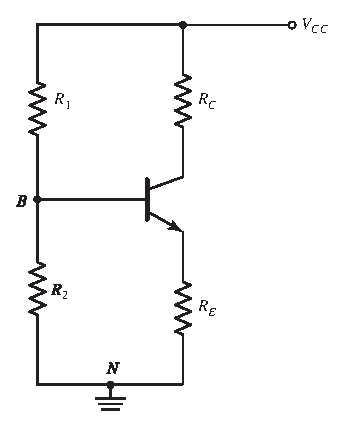
\includegraphics{chap3/S3-EE-03-046.eps}

\medskip
\colorbox{lightgray}{{\bf Fig.\,4.13:} {\em Voltage divider bias circuit}}
\end{figure}
\end{minipage}
\qquad\qquad
\begin{minipage}[b]{6cm}
\begin{figure}[H]
\centering
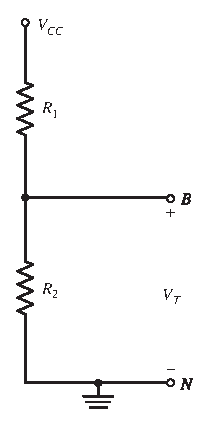
\includegraphics{chap3/S3-EE-03-047.eps}

\medskip
\colorbox{lightgray}{{\bf Fig.\,4.14:} {\em Voltage divider network}}
\end{figure}
\end{minipage}
\end{center}

Consider the voltage divider network shown in Fig.~4.14. $V_{T}$ is the voltage across $R_{2}$. Using voltage division rule we get
\begin{equation}
V_{T}=\frac{V_{CC}R_{2}}{R_{1}+R_{2}}\label{eq4.26}
\end{equation}
$V_{T}$ is the Thevenin's voltage.

\vskip .1cm

To find $R_{T}$ we have to connect $V_{CC}$ point to ground as shown in Fig.~\ref{fig4.15}.

\vskip .1cm

$R_{T}$ is the equivalent resistance between the terminals $B$ and $N$.
\begin{equation}
R_{T}=R_{1} \,||\, R_{2}=\frac{R_{1}R_{2}}{R_{1}+R_{2}}\label{eq4.27}
\end{equation}
$R_{T}$ is the Thevenin's resistance.
\setcounter{figure}{14}
\begin{figure}[H]
\centering
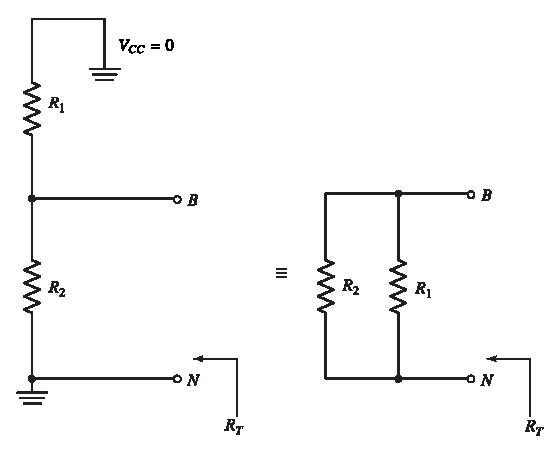
\includegraphics{chap3/S3-EE-03-048.eps}
\caption{Circuit to find $R_{T}$}\label{fig4.15}
\end{figure}

The Thevenin's equivalent circuit of voltage divider network of Fig.~4.14 between the points $B$ and $N$ is shown in Fig.~\ref{fig4.16}.
\begin{figure}[H]
\centering
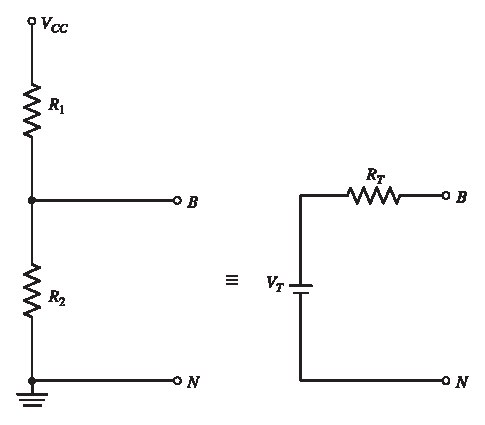
\includegraphics{chap3/S3-EE-03-049.eps}
\caption{Thevenin's equivalent of voltage divider network}\label{fig4.16}
\end{figure}

Now let us replace the voltage divider network in Fig.~4.13 with its Thevenin's equivalent circuit between the terminals $B$ and $N$ as shown in Fig.~\ref{fig4.17}.
\begin{figure}[H]
\centering
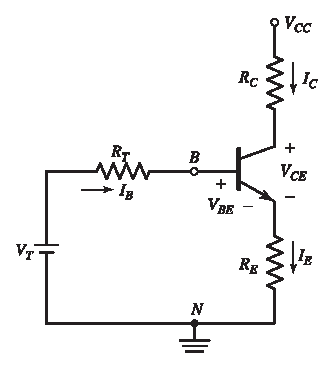
\includegraphics{chap3/S3-EE-03-050.eps}
\caption{Voltage divider bias with Thevenin's equivalent circuit}\label{fig4.17}
\end{figure}

Applying Kirchhoff's Voltage Law to the base-emitter circuit of Fig.~\ref{fig4.17} we have
\begin{align}
V_{T} &= R_{T}I_{B}+V_{BE}+I_{E}R_{E}\label{eq4.28}\\[3pt]
\text{But}\qquad I_{E} &= I_{B}+I_{C}=I_{B}+h_{FE}I_{B}\notag\\[3pt]
\Longrightarrow\quad I_{E} &= (1+h_{FE})I_{B}\notag
\end{align}

Using this relation in Eqn.~\eqref{eq4.28} we have
\begin{align}
V_{T}-V_{BE} &= I_{B}[R_{T}+(1+h_{FE})R_{E}]\notag\\[3pt]
I_{B} &= \frac{V_{T}-V_{BE}}{R_{T}+(1+h_{FE})R_{E}}\label{eq4.29}
\end{align}

Once $I_{B}$ is known, the collector current $I_{C}$ is obtained by
\begin{equation}
I_{C}=h_{FE}I_{B}\label{eq4.30}
\end{equation}

$V_{CE}$ can be obtained by applying Kirchhoff's Voltage Law to collector-emitter circuit
\begin{align}
V_{CC} &= I_{C}R_{C}+V_{CE}+I_{E}R_{E}\notag\\[3pt]
V_{CE} &= V_{CC}-I_{C}R_{C}-I_{E}R_{E}\label{eq4.31}
\end{align}

\begin{example}\label{exam4.14}
Analyse the voltage divider bias circuit shown below to determine emitter voltage $V_{E}$, collector voltage $V_{C}$, base voltage $V_{B}$, collector current $I_{C}$ and collector to emitter voltage $V_{CE}$. Assume Silicon transistor with $V_{BE}=0.7\text{V}$. Draw the DC load line and mark the $Q$ point.
\begin{figure}[H]
\centering
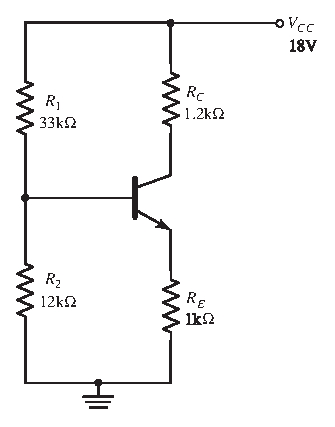
\includegraphics[scale=1.05]{chap3/S3-EE-03-IN023.eps}
\end{figure}
\end{example}

\begin{solution}
Let us redraw the given circuit with all voltages and currents marked as shown below.
\begin{figure}[H]
\centering
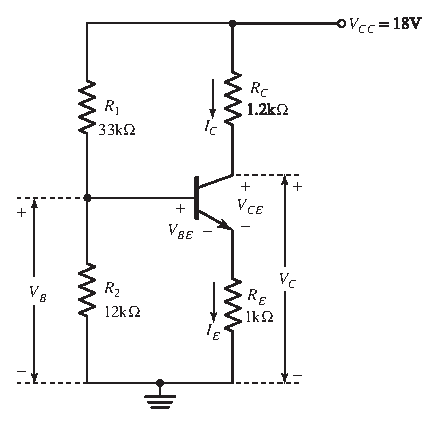
\includegraphics[scale=1.05]{chap3/S3-EE-03-IN024.eps}
\end{figure}

Since $h_{FE}$ is not given we cannot find $I_{B}$. Therefore we have to use approximate analysis neglecting $I_{B}$.
\begin{align*}
V_{B} &= \frac{V_{CC}R_{2}}{R_{1}+R_{2}}=\frac{18\text{V}\times 12 k\Omega}{33 k\Omega + 12 k\Omega}=4.8 \text{V}\\[7pt]
V_{E} &= V_{B}-V_{BE}= 4.8\text{V}-0.7\text{V}= 4.1\text{V}\\[7pt]
I_{E} &= \frac{V_{E}}{R_{E}}= \frac{4.1\text{V}}{1 k\Omega}= 4.1\text{\,mA}\\[3pt]
I_{C}\simeq I_{E} &= 4.1\text{\,mA}\\[7pt]
V_{CE} &= V_{CC}-I_{C}(R_{C}+R_{E})\\[3pt]
&= 18\text{V}-(4.1\text{\,mA})(1.2 k\Omega + 1k\Omega)\\[3pt]
&= 8.98\text{V}\\[3pt]
V_{C} &= V_{CE}+I_{E}R_{E}\\[3pt]
&= 8.98\text{V}+(4.1 \text{\,mA})(1 k\Omega)\\[3pt]
&= 13.08\text{V}\\[3pt]
Q(V_{CE},I_{C}) &= Q(8.98\text{V}, 4.1 \text{\,mA})
\end{align*}

The $Q$ point is marked on the DC load line in the figure shown below.
\begin{figure}[H]
\centering
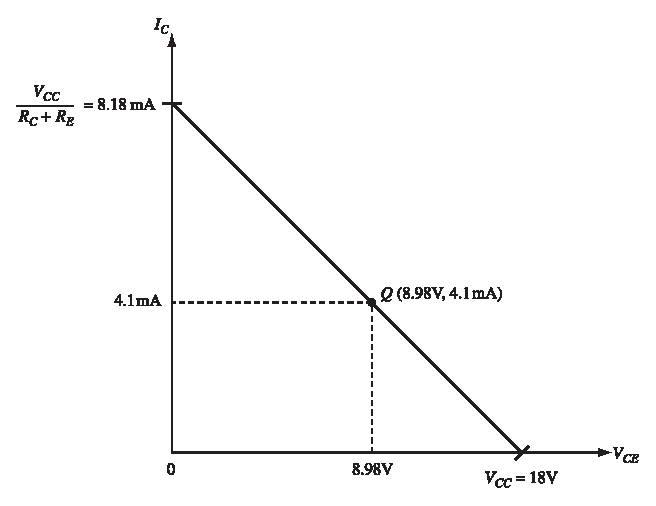
\includegraphics{chap3/S3-EE-03-IN025.eps}
\end{figure}
\vskip -1cm
\end{solution}

\eject

\begin{example}\label{exam4.15}
A voltage divider bias circuit has $V_{CC}=15\text{V}$, $R_{C}=2.7 k\Omega$, $R_{E}=2.2 k\Omega$, $R_{1}=22 k\Omega$, $R_{2}=12 k\Omega$. Calculate $V_{E}$, $V_{C}$, $I_{C}$ and $V_{CE}$. Draw the DC load line and mark the $Q$ point. Take $V_{BE}=0.7\text{V}$.
\end{example}

\begin{solution}
Given,
\begin{align*}
 V_{CC} &= 15\text{V},\quad R_{C}=2.7 k\Omega,\quad R_{E}=2.2 k\Omega,\\[3pt]
 R_{1} &= 22 k\Omega,\quad R_{2}=12 k\Omega,\quad V_{BE}=0.7 \text{V}
\end{align*}

Since $h_{FE}$ is not given, we have to use approximate analysis neglecting $I_{B}$.
\begin{align*}
V_{B} &= \frac{V_{CC}R_{2}}{R_{1}+R_{2}}=\frac{15\text{V}\times 12 k\Omega}{22 k\Omega+12 k\Omega}=5.29\text{V}\\[3pt]
V_{E} &= V_{B}-V_{BE}=5.29\text{V}-0.7\text{V}=4.59\text{V}\\[3pt]
I_{E} &= \frac{V_{E}}{R_{E}}=\frac{4.59\text{V}}{2.2 k\Omega}=2.09\text{\,mA}\\
I_{C} &\simeq I_{E}=2.09\text{\,mA}\\[3pt]
V_{CE} &= V_{CC}-I_{C}[R_{C}+R_{E}]\\[3pt]
&= 15\text{V}-(2.09\text{\,mA})\,[2.7\,k\Omega+2.2\,k\Omega]=4.76\text{V}\\[3pt]
V_{C} &= V_{CE}+V_{E}=4.76\text{V}+4.59\text{V}= 9.35\text{V}\\[3pt]
Q(V_{CE},I_{C}) &= Q(4.76\text{V}, 2.09\text{\,mA})
\end{align*}
The dc load line is shown in the following figure.
\begin{figure}[H]
\centering
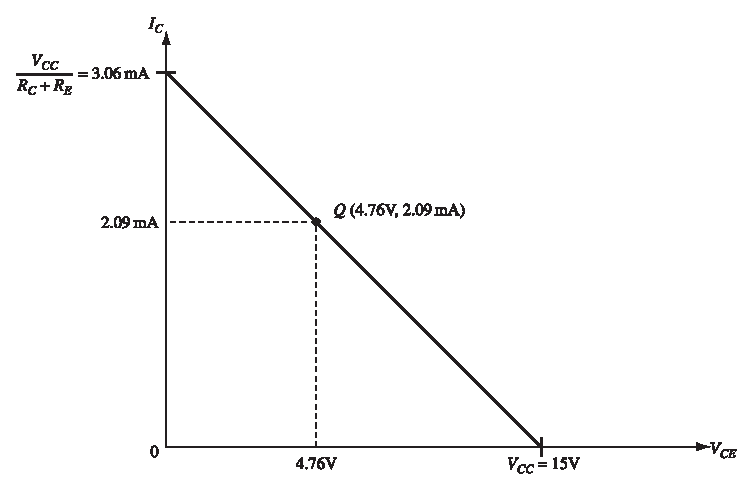
\includegraphics[scale=.93]{chap3/S3-EE-03-IN026.eps}
\end{figure}
\vskip -1cm
\end{solution}

\eject

\begin{example}\label{exam4.16}
A voltage divider bias circuit has $V_{CC}=18\text{V}$, $R_{1}=33 k\Omega$, $R_{2}=12 k\Omega$, $R_{E}=1 k\Omega$, $R_{C}=1.2 k\Omega$, $h_{FE}=50$. Taking $V_{BE}=0.7\text{V}$, find $V_{E}$, $I_{C}$, $V_{CE}$ and $V_{C}$. Draw the DC load line and locate the $Q$ point.
\end{example}

\begin{solution}
Given,
\begin{align*}
V_{CC} &= 18\text{V}, \ V_{BE}=0.7\text{V}, \ h_{FE}=50,\\[3pt]
R_{1} &= 33 k\Omega, \ R_{2}=12 k\Omega, \ R_{C}=1.2 k\Omega, \ R_{E}=1 k\Omega
\end{align*}

Since $h_{FE}$ is given, $I_{B}$ can be calculated. Hence we can use exact analysis.
\begin{align*}
V_{T} &= \frac{V_{CC}R_{2}}{R_{1}+R_{2}}=\frac{18\text{V}\times 12 k\Omega}{33 k\Omega +12 k\Omega}=4.8\text{V}\\[4pt]
R_{T} &= \frac{R_{1}R_{2}}{R_{1}+R_{2}}=\frac{33 k\Omega \times 12 k\Omega}{33 k\Omega + 12 k\Omega}=8.8 k\Omega\\[7pt]
I_{B} &= \frac{V_{T}-V_{BE}}{R_{T}+(1+h_{FE})R_{E}}\\[4pt]
&= \frac{4.8\text{V}-0.7\text{V}}{8.8 k\Omega+(1+50)(1 k\Omega)}\\[4pt]
&= 0.0686\text{\,mA}=68.6\,\mu\text{\,A}\\[4pt]
I_{C} &= h_{FE}I_{B}=(50)(0.0686\text{\,mA})=3.43\text{\,mA}\\[4pt]
I_{E} &= I_{B}+I_{C}=(0.0686\text{\,mA}+3.43\text{\,mA})=3.5\text{\,mA}\\[4pt]
V_{E} &= I_{E}R_{E}=(3.5\text{\,mA})(1 k\Omega)=3.5\text{V}\\[7pt]
V_{CE} &= V_{CC}-I_{C}R_{C}-I_{E}R_{E}\\[4pt]
&= 18\text{V}-(3.43\text{\,mA})(1.2 k\Omega)-(3.5\text{\,mA})(1 k\Omega)=10.38 \text{V}\\[4pt]
V_{C} &= V_{CE}+V_{E}\\[4pt]
&= 10.38\text{V}+3.5\text{V}\\[4pt]
&= 13.88\text{V}\\[4pt]
Q(V_{CE},I_{C}) &= Q(10.38\text{V}, \ 3.43\text{\,mA})
\end{align*}
The dc load line is shown in the following figure.
\begin{figure}[H]
\centering
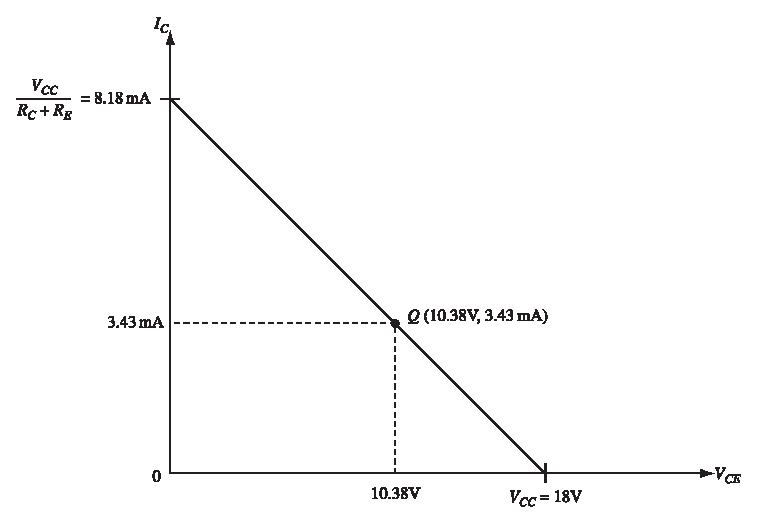
\includegraphics{chap3/S3-EE-03-IN027.eps}
\end{figure}
\vskip -1cm
\end{solution}

\medskip

\begin{example}\label{exam4.17}
The voltage divider bias circuit has $V_{CC}=15\text{V}$, $R_{1}=6.8 k\Omega$, $R_{2}=3.3 k\Omega$, $R_{C}=900\Omega$, $R_{E}=900\Omega$ and $h_{FE}=50$, $V_{BE}=0.7\text{V}$. Find the levels of $V_{E}$, $I_{B}$, $I_{C}$, $V_{CE}$ and $V_{C}$. Draw the DC load line and mark the $Q$ point on that.
\end{example}

\begin{solution}
Given,
\begin{align*}
V_{CC} &= 15\text{V},\quad V_{BE}=0.7\text{V},\quad R_{1}=6.8 k\Omega,\\[3pt]
R_{2} &= 3.3\,k\Omega,\quad R_{C}=900\,\Omega = 0.9\,k\Omega,\\[3pt]
R_{E} &= 900\Omega = 0.9 k\Omega,\quad h_{FE}=50
\end{align*}
Since $h_{FE}$ is given let us use exact analysis.
\begin{align*}
V_{T} &= \frac{V_{CC}R_{2}}{R_{1}+R_{2}}=\frac{15\text{V}\times 3.3 k\Omega}{6.8 k\Omega + 3.3 k\Omega}=4.9\text{V}\\[3pt]
R_{T} &= \frac{R_{1}R_{2}}{R_{1}+R_{2}}=\frac{6.8 k\Omega\times 3.3 k\Omega}{6.8 k\Omega + 3.3 k\Omega}=2.22 k\Omega\\[3pt]
I_{B} &= \frac{V_{T}-V_{BE}}{R_{T}+(1+ h_{FE})R_{E}}=\frac{4.9\text{V}-0.7\text{V}}{2.22 k\Omega + (1+50)(0.9 k\Omega)}=0.0873\text{\,mA}\\[3pt]
I_{C} &= h_{FE}I_{B}=50\times 0.0873\text{\,mA}=4.365\text{\,mA}\\[3pt]
I_{E} &= I_{B}+I_{C}=0.0873\text{\,mA}+4.365\text{\,mA}=4.45\text{mA}\\[7pt]
V_{E} &= I_{E}R_{E}=(4.45\text{\,mA})(0.9 k\Omega)=4\text{V}\\[3pt]
V_{CE} &= V_{CC}-I_{C}R_{C}-V_{E}\\[3pt]
&= 15\text{V}-(4.365\text{\,mA})(0.9 k\Omega)-4\text{V}=7.07\text{V}\\[3pt]
V_{C} &= V_{CE}+V_{E}\\[3pt]
&= 7.07\text{V}+4\text{V}\\[3pt]
&= 11.07\text{V}\\[3pt]
Q(V_{CE},I_{C}) &= Q(7.07\text{V}, 4.365\text{\,mA})
\end{align*}
\begin{figure}[H]
\centering
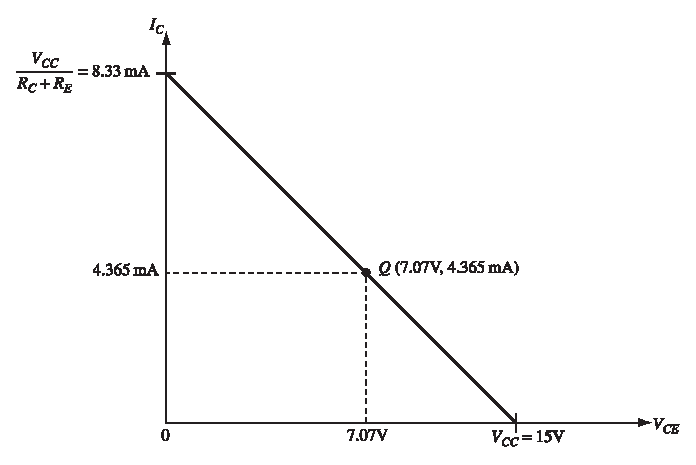
\includegraphics{chap3/S3-EE-03-IN028.eps}
\end{figure}
\vskip -1cm
\end{solution}

\section{Design of voltage divider bias circuit}\label{sec4.9}
\index{Voltage divider bias!design of}

The design of voltage divider bias circuit involves the calculation of $R_{1}$, $R_{2}$, $R_{E}$ and $R_{C}$ for a given $V_{CC}$, $V_{CE}$, $I_{C}$, $V_{BE}$ and $h_{FE}$. Following points are to noted while designing the circuit.
\begin{itemize}
\item $I_{2}$ is selected to be much larger than $I_{B}$. This makes $V_{B}$ a stable quantity largely unaffected by the transistor $h_{FE}$ value. As a thumb rule, $I_{2}$ is selected to be equal to one tenth of $I_{C}$. i.e.,
\begin{equation}
I_{2}=\frac{I_{C}}{10}\label{eq4.32}
\end{equation}
This gives reasonably large value for $R_{1}$ and $R_{2}$ while still keeping $I_{2}\gg I_{B}$. Large values of $R_{1}$ and $R_{2}$ are desirable to achieve high input impedance.

\item $V_{E}$ should be selected much larger than $V_{BE}$, i.e., $V_{E}\gg V_{BE}$. This is because $V_{BE}$ varies from transistor to transistor. Also $V_{BE}$ varies with temperature. If $V_{E}\gg V_{BE}$, the effect of $V_{BE}$ variation on the circuit bias condition is minimized. The level of $V_{E}$ in the range $3\text{V}-5\text{V}$ is reasonable.

\item $R_{E}$ is calculated using
\begin{equation}
R_{E}=\frac{V_{E}}{I_{C}}\label{eq4.33}
\end{equation}

\item $R_{2}$ is calculated using
\begin{align}
R_{2} &= \frac{V_{B}}{I_{2}}\label{eq4.34}\\
\text{where}\quad V_{B} &= V_{BE}+V_{E}\notag
\end{align}

\item $R_{1}$ is calculated from the relation
\begin{align}
V_{CC} &= I_{1}R_{1}+I_{2}R_{2}=I_{2}R_{1}+V_{B}\quad (\because \ I_{1}\simeq I_{2})\notag\\[4pt]
\Longrightarrow\quad R_{1} &= \frac{V_{CC}-V_{B}}{I_{2}}\label{eq4.35}
\end{align}

\item $R_{C}$ is obtained from the relation
\begin{align}
V_{CC} &= I_{C}R_{C}+V_{CE}+V_{E}\\[4pt]
\Longrightarrow\quad R_{C} &= \frac{V_{CC}-V_{CE}-V_{E}}{I_{C}}\label{eq4.36}
\end{align}
\end{itemize}

\begin{example}\label{exam4.18}
Design a voltage divider bias circuit to have $V_{CE}=V_{E}=5\text{V}$ and $I_{C}=5\text{\,mA}$, when the supply voltage is $15\text{V}$. Assume the transistor $h_{FE}$ as $100$ and $V_{BE}=0.7\text{V}$.
\end{example}

\begin{solution}
\begin{align*}
R_{E} &= \frac{V_{E}}{I_{E}}\simeq \frac{V_{E}}{I_{C}}\\[4pt]
&= \frac{5\text{V}}{5\text{\,mA}}\\[4pt]
&= 1 k\Omega\\[7pt]
R_{C} &= \frac{V_{CC}-V_{CE}-V_{E}}{I_{C}}\\[4pt]
&= \frac{15\text{V}-5\text{V}-5\text{V}}{5\text{\,mA}}\\[4pt]
&= 1 k\Omega\\[7pt]
I_{2} &= \frac{I_{C}}{10}=\frac{5\text{\,mA}}{10}=0.5\text{\,mA}\\[4pt]
V_{B} &= V_{BE}+V_{E}\\[4pt]
&= 0.7\text{V}+5\text{V}\\[4pt]
&= 5.7\text{V}\\[7pt]
R_{1} &= \frac{V_{CC}-V_{B}}{I_{2}}\\[4pt]
&= \frac{15\text{V}-5.7\text{V}}{0.5\text{\,mA}}\\[4pt]
&= 18.6\,k\Omega\\[7pt]
R_{2} &= \frac{V_{B}}{I_{2}}\\[4pt]
&= \frac{5.7\text{V}}{0.5\text{\,mA}}\\[4pt]
&= 11.4\,k\Omega
\end{align*}

The voltage divider bias circuit with designed component values is shown below.
\begin{figure}[H]
\centering
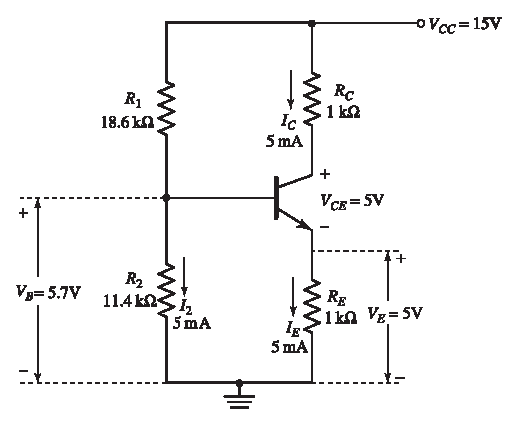
\includegraphics[scale=1.05]{chap3/S3-EE-03-IN029.eps}
\end{figure}
\vskip -1cm
\end{solution}

\eject

\begin{example}\label{exam4.19}
Design a voltage divider bias circuit to operate from a $12\text{V}$ supply. The bias conditions are to be $V_{CE}=3\text{V}$, $V_{E}=5\text{V}$ and $I_{C}=1\text{\,mA}$. Take $V_{BE}=0.7\text{V}$.
\end{example}

\begin{solution}
Given,
\begin{align*}
R_{E} &= \frac{V_{E}}{I_{E}}\simeq \frac{V_{E}}{I_{C}}=\frac{5\text{V}}{1\text{\,mA}}=5\, k\Omega\\[3pt]
R_{C} &= \frac{V_{CC}-V_{CE}-V_{E}}{I_{C}}
= \frac{12\text{V}-3\text{V}-5\text{V}}{1\text{\,mA}}\\[3pt]
&= 4\, k\Omega\\[3pt]
I_{2} &= \frac{I_{C}}{10}=\frac{1\text{\,mA}}{10}=0.1\text{\,mA}\\[3pt]
V_{B} &= V_{BE}+V_{E}= 0.7\text{V}+5\text{V}\\[3pt]
&= 5.7\text{V}\\[3pt]
R_{1} &= \frac{V_{CC}-V_{B}}{I_{2}}\\[3pt]
&= \frac{12\text{\,V}-5.7\text{V}}{0.1\text{\,mA}}=63\, k\Omega\\[3pt]
R_{2} &= \frac{V_{B}}{I_{2}}= \frac{5.7\text{V}}{0.1\text{\,mA}}=57\, k\Omega
\end{align*}
The voltage divider bias circuit with designed component values is shown below.
\begin{figure}[H]
\centering
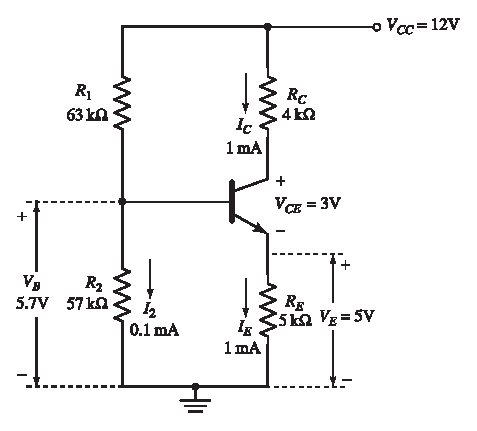
\includegraphics[scale=1.05]{chap3/S3-EE-03-IN030.eps}
\end{figure}
\vskip -1cm
\end{solution}

\begin{example}\label{exam4.20}
Design a voltage divider bias circuit to have $V_{CE}=10\text{V}$ and $I_{C}=1\text{\,mA}$. The supply voltage is $V_{CC}=30\text{V}$ and $V_{BE}=0.7\text{V}$.
\end{example}

\begin{solution}
Given,
\begin{align*}
V_{CC} &= 30\text{V},\quad V_{CE}=10\text{V}\\[3pt]
V_{BE} &= 0.7\text{V},\quad I_{C}=1\text{\,mA}
\end{align*}
Select $V_{E}=5\text{V}$
\begin{align*}
R_{E} &= \frac{V_{E}}{I_{E}}\simeq \frac{V_{E}}{I_{C}}=\frac{5\text{V}}{1\text{\,mA}}=5 k\Omega\\[3pt]
R_{C} &= \frac{V_{CC}-V_{CE}-V_{E}}{I_{C}}\\[3pt]
&= \frac{30\text{V}-10\text{V}-5\text{V}}{1\,\text{mA}}= 15 k\Omega\\[3pt]
I_{2} &= \frac{I_{C}}{10}=\frac{1\text{\,mA}}{10}=0.1\text{\,mA}\\[3pt]
V_{B} &= V_{BE}+V_{E}=0.7\text{V}+5\text{V}=5.7\text{V}\\[3pt]
R_{1} &= \frac{V_{CC}-V_{B}}{I_{2}}=\frac{30\text{V}-5.7\text{V}}{0.1\text{\,mA}}=243 k\Omega\\[3pt]
R_{2} &= \frac{V_{B}}{I_{2}}=\frac{5.7\text{V}}{0.1\text{\,mA}}=57 k\Omega
\end{align*}
The voltage divider bias circuit with designed component values is shown below.
\begin{figure}[H]
\centering
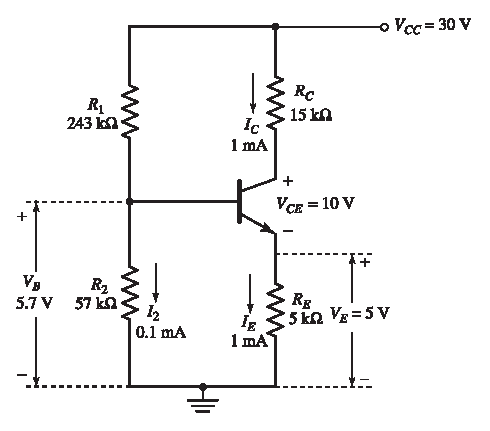
\includegraphics[scale=1.05]{chap3/S3-EE-03-IN031.eps}
\end{figure}
\vskip -1cm
\end{solution}

\eject

\begin{example}\label{exam4.21}
A voltage divider bias circuit with $V_{CC}=20\text{V}$ and $R_{C}=6\,k\Omega$ uses a transistor with $h_{FE}=80$. Calculate suitable resistor values to give $V_{CE}=8\text{V}$. Take $V_{BE}=0.7\text{V}$.
\end{example}

\begin{solution}
Given,
$$
V_{CC}=20\text{V},\quad V_{CE}=8\text{V},\quad h_{FE}=80,\quad R_{C}=6\,k\Omega
$$
Select $V_{E}=5\text{V}$
\begin{align*}
R_{C} &= \frac{V_{CC}-V_{CE}-V_{E}}{I_{C}}\\[3pt]
\Longrightarrow\quad I_{C} &= \frac{V_{CC}-V_{CE}-V_{E}}{R_{C}}\\[3pt]
I_{C} &= \frac{20\text{V}-8\text{V}-5\text{V}}{6 k\Omega}=1.167\text{\,mA}\\[3pt]
I_{2} &=\frac{I_{C}}{10}=\frac{1.167\text{\,mA}}{10}=0.1167\text{\,mA}\\[3pt]
R_{E} &= \frac{V_{E}}{I_{E}}\simeq \frac{V_{E}}{I_{C}}=\frac{5\text{V}}{1.167\text{\,mA}}=4.28\,k\Omega\\[3pt]
V_{B} &= V_{BE}+V_{E}= 0.7\text{V}+5\text{V}= 5.7\text{V}\\[3pt]
R_{1} &= \frac{V_{CC}-V_{B}}{I_{2}}=\frac{20\text{V}-5.7\text{V}}{0.1167\text{\,mA}}=122.54\,k\Omega\\[3pt]
R_{2} &= \frac{V_{B}}{I_{2}}=\frac{5.7\text{V}}{0.1167\text{\,mA}}=48.84\,k\Omega
\end{align*}
The voltage divider bias circuit with designed component values is shown below.
\begin{figure}[H]
\centering
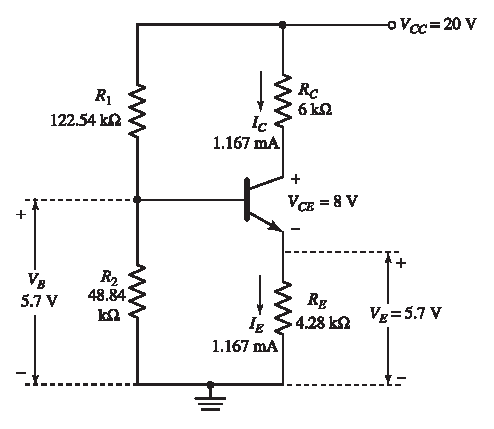
\includegraphics[scale=1.02]{chap3/S3-EE-03-IN032.eps}
\end{figure}
\vskip -1cm
\end{solution}

\eject

\section{Thermal stability of bias circuits}\label{sec4.10}

Many transistor circuits are required to operate over a wide temperature range. Hence thermal stability of a bias circuit is an important aspect. Thermal stability\index{Thermal stability} checks how stable $I_{C}$ and $V_{CE}$ ($Q$ point) remain when the circuit temperature changes.

Following are the factors which degrades the thermal stability\index{Biasing circuits!thermal stability} of a biasing circuit.
\begin{enumerate}
\item The collector-base reverse saturation current $I_{CB0}$, doubles for every $10^{\circ}$C rise in temperature.

\item The base-emitter voltage, $V_{BE}$, changes by approximately $-1.8$\,mV/$^{\circ}$C, for a silicon transistor.

\item The dc current gain, $h_{FE}$, of the transistor changes with temperature. The value of $h_{FE}$ also differs from one transistor to another transistor.
\end{enumerate}

All these factors causes the drift in $Q$ point as shown in Fig.~\ref{fig4.18}. Note that, as the temperature increases, the $Q$ point shifts up the dc load line.
\begin{figure}[H]
\centering
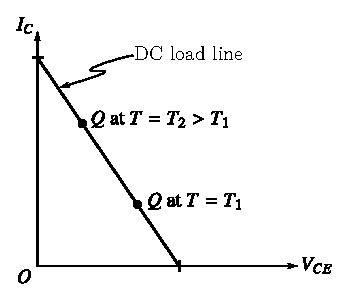
\includegraphics{chap3/fig3.18.eps}
\caption{Effect of temperature on $Q$ point}\label{fig4.18}
\end{figure}

\medskip

\section[Thermal stability of $Q$ point in Base-Bias]{Thermal stability of \boldmath$Q$ point in Base-Bias}\label{sec4.11}

We have the following relations for base-bias circuit (Refer. Fig.~\ref{fig4.9}).
\begin{align}
I_{B} &\approx \frac{V_{CC}}{R_{B}}=\text{constant}\label{eq4.38}\\[7pt]
I_{C} &= h_{FE}I_{B}\label{eq4.39}\\
V_{CE} &= V_{CC}-I_{C}R_{C}\label{eq4.40}
\end{align}

If $I_{C}$ increases due to increase in temperature, $I_{C}R_{C}$ increases and hence $V_{CE}$ decreases. This causes the $Q$ point to shift up the dc load line as shown in Fig.~\ref{fig4.18}.

Hence base-bias circuit has poor thermal stability of $Q$ point.

\section[Thermal stability of $Q$ point in voltage divider bias circuit]{Thermal stability of \boldmath$Q$ point in voltage divider bias circuit}

From Eqn.~\eqref{eq4.28} of voltage divider bias circuit (Refer Fig.~\ref{fig4.17}), we have
\begin{align}
& V_{T} = I_{B}R_{T}+V_{BE}+I_{E}R_{E}\notag\\[3pt]
\text{or}\quad & V_{T}-V_{BE}=I_{B}R_{T}+I_{E}R_{E}\label{eq4.41}
\end{align}

In Eqn.~\eqref{eq4.41}, $V_{T}-V_{BE}\approx$ constant. When the temperature increases,
\begin{itemize}
\item $I_{C}$ increases.

\item $I_{E}R_{E}$ increases.

\item Since, $V_{T}-V_{BE}=\text{constant}$, $I_{B}R_{T}$ should decrease.

\item Since $R_{T}$ is a constant, $I_{B}$ should decrease.

\item Hence $I_{C}$ decreases.
\end{itemize}

Note that an increase in $I_{C}$ is reflected in an increase in $I_{E}R_{E}$ which inturn causes $I_{C}$ to decrease. 

Hence the voltage divider bias circuit has good stability of $Q$ point.

\smallskip
\begin{center}
\rule{5cm}{1pt}\\[-2pt]
{\bf Exercise Problems}\\[-4pt]
\rule{5cm}{1pt}
\end{center}

\begin{enumerate}
\renewcommand{\labelenumi}{\bf\theenumi.}
\item A base bias circuit has $V_{CC}=25\text{V}$, $R_{B}=330k\Omega$, $R_{C}=3.9k\Omega$ and $V_{CE}=12\text{V}$. Calculate the value of $h_{FE}$. Determine the new $V_{CE}$ level when a new transistor with $h_{FE}=125$ is substituted.

\item Design a base bias circuit to have $V_{CE}=6\text{V}$ and $I_{C}=6\text{mA}$. The supply voltage is 12\,V and $h_{FE}$ of the transistor is 100.

\item A base bias circuit has $V_{CC}=20\text{V}$, $R_{C}=6.8\Omega$ and $h_{FE}=125$. Calculate the value of $R_{B}$ to give $V_{CE}=10\text{V}$.

\item A voltage divider bias circuit has the following data : $V_{CC}=18\text{V}$, $R_{1}=39\,k\Omega$, $R_{2}=10\,k\Omega$, $R_{C}=1\,k\Omega$. Calculate the values of $I_{C}$, $V_{C}$, $V_{CE}$ and $V_{E}$. Draw the $dc$ load line and locate the $Q$ point.

\item A voltage divider bias circuit has $V_{CC}=20\text{V}$, $R_{1}=39\,k\Omega$, $R_{2}=12\,k\Omega$, $R_{C}=1\,k\Omega$, $R_{E}=1.2\,k\Omega$, $h_{FE}=75$. Calculate $I_{B}$, $I_{C}$, $I_{E}$, $V_{CE}$ and $V_{C}$. Draw the dc load line and locate the $Q$ point.

\item Design the voltage divider bias circuit to have $V_{CE}=V_{E}=6\text{V}$, $I_{C}=6\text{mA}$ and $V_{CC}=16\text{V}$. Assume silicon transistor with $h_{FE}=100$.
\end{enumerate}


